% allocate 9 pages
\chapter{Evaluation} 
\label{sec:evaluation}
This chapter analyses two research questions proposed in \Cref{section:motivation} through quantitative and qualitative methods. The first question is addressed in \Cref{sec:eval-prompt}, where prompting model performance in a few-shot learning scenario is compared. The second question is explored in \Cref{sec:eval-backdoor}, demonstrating the vulnerability of each prompting model to different backdoor attack settings. Additionally, \Cref{sec:eval-success} evaluates how the success criteria for both the core project and its extensions are met.

\section{Prompting Model Performance Analysis} \label{sec:eval-prompt}
\subsection{Prompt \& Verbaliser Designs}
\subsubsection{Designs In Manual Prompting} \label{sec:eval-manul-prompt}
For each of the six datasets, four to six manual prompt-and-verbaliser pairs are chosen from either the Public Pool of Prompts \cite{Bach22OPP} or previous literature on prompting \cite{Gao20PM, Lei22}. The performance of the pairs are compared under the same $K = 16$ few-shot scenario. Detailed results can be found in \Cref{tab:manual_select}. The mean and standard deviation of the classification performance score (Accuracy or F1 score) are computed across five independent runs with different random seeds (e.g., \texttt{seed $\in$ \{13, 21, 42, 87, 100\}}) using the same experimental setting. 

\begin{table}[!ht]
\centering
\adjustbox{max width=\hsize}{
	\begin{tabular}{l | c | c | l | c | c}
	\toprule                      
	\multicolumn{3}{c}{SST2}                      
	& \multicolumn{3}{c}{QNLI} \\
	\textbf{Prompt Design} & \textbf{Answer $\mapsto$ Label} & \textbf{Accuracy}
    & \textbf{Prompt Design} & \textbf{Answer $\mapsto$ Label} & \textbf{Accuracy}\\
	\midrule  
	% SST2
	\multirow{6}{*}{\texttt{<sentence> . It was <mask> .}}
    & {\texttt{terrible} $\mapsto$ 0, \texttt{great} $\mapsto$ 1}
    & $86.0 \pm 2.7$
	% QNLI 
	& \texttt{<question> ? <mask> , <sentence> .}      
	& \multirow{5}{*}{\{\texttt{Yes} $\mapsto$ 0,}
    & $64.5 \pm 4.8$
	\\ 
    % SST2
    & {\texttt{bad} $\mapsto$ 0, \texttt{good} $\mapsto$ 1}
    & $\boldsymbol{86.9 \pm 1.6}$ 
	% QNLI 
	& \texttt{<question> . <mask> , <sentence> .}      
	& \multirow{5}{*}{ \texttt{No} $\mapsto$ 1\}}
    & $60.5 \pm 2.3$
    \\
    % SST2
    & {\texttt{dog} $\mapsto$ 0, \texttt{cat} $\mapsto$ 1}
    & $84.7 \pm 3.4$
	% QNLI 
	& \texttt{<question> ? <mask> <sentence> .}   
	&  
    & $68.7 \pm 3.2$
	\\
    % SST2
    & {\texttt{cat} $\mapsto$ 0, \texttt{dog} $\mapsto$ 1}
    & $68.7 \pm 6.9$
	% QNLI 
	& \texttt{<sentence> ? <mask> , <question> .}       
	&  
    & $\boldsymbol{74.1 \pm 1.2}$
    \\
    % SST2
    & {\texttt{great} $\mapsto$ 0, \texttt{terrible} $\mapsto$ 1}  
    & $67.4 \pm 5.0$
	% QNLI 
	& \texttt{<question> <mask> <sentence>}       
	&  
    & $50.0 \pm 0.2$
    \\
    % SST2 
    &   
    & 
	% QNLI 
	& \texttt{<sentence> ? <mask> , <question>}       
	&  
    & $66.7 \pm 10.2$ \\
    \midrule
	\multicolumn{3}{c}{MNLI-Matched}               
	& \multicolumn{3}{c}{MNLI-Mismatched} \\
	\textbf{Prompt Design} & \textbf{Answer $\mapsto$ Label} & \textbf{Accuracy}
    & \textbf{Prompt Design} & \textbf{Answer $\mapsto$ Label} & \textbf{Accuracy}
	\\
	\midrule
        % matched
        \texttt{<premise> ? <mask> , <hypothesis> .}
        & \multirow{4}{*}{\{\texttt{Yes} $\mapsto$ 0,}
        & $\boldsymbol{60.2 \pm 3.7}$
        % mismatched
        & \texttt{<premise> ? <mask> , <hypothesis> .}
        & \multirow{4}{*}{\{\texttt{Yes} $\mapsto$ 0,}
        & $\boldsymbol{60.2 \pm 2.7}$
        \\
        % matched
        \texttt{<premise> . <mask> , <hypothesis> .}
        & \multirow{4}{*}{\texttt{Maybe} $\mapsto$ 1,}
        & $58.6 \pm 4.8$
        % mismatched
        & \texttt{<premise> . <mask> , <hypothesis> .}
        & \multirow{4}{*}{\texttt{Maybe} $\mapsto$ 1,}
        & $56.3 \pm 1.5$
        \\	
        % matched
        \texttt{<premise> ? <mask> <hypothesis> .}
        & \multirow{4}{*}{\texttt{No} $\mapsto$ 2\}}
        & $55.6 \pm 1.7$
        % mismatched
        & \texttt{<premise> ? <mask> <hypothesis> .}
        & \multirow{4}{*}{ \texttt{No} $\mapsto$ 2\}}
        & $58.4 \pm 1.1$
        \\
        % matched
        \texttt{<hypothesis> ? <mask> , <premise> .}
        & 
        &  $51.9 \pm 4.2$
        % mismatched
        & \texttt{<hypothesis> ? <mask> , <premise> .}
        & 
        & $57.9 \pm 0.8$
        \\
        % matched
        \texttt{<premise> <mask> <hypothesis>}
        & 
        & $51.2 \pm 4.2$
        % mismatched
        & \texttt{<premise> <mask> <hypothesis>}
        & 
        & $49.4 \pm 2.4$
        \\
        % matched
        \texttt{<hypothesis> ? <mask> , <premise>}
        &
        & $52.4 \pm 2.9$
        % mismatched
        & \texttt{<hypothesis> ? <mask> , <premise>}
        & 
        & $56.0\pm 1.0$ \\
        \midrule                   
	\multicolumn{3}{c}{ENRON-SPAM}                      
	& \multicolumn{3}{c}{TWEETS-HATE-OFFENSIVE} \\
	\textbf{Prompt Design} & \textbf{Answer $\mapsto$ Label} & \textbf{F1 score}
    & \textbf{Prompt Design} & \textbf{Answer $\mapsto$ Label} & \textbf{F1 score}
	\\
        \midrule
        % enron-spam
        \texttt{<mask> : <text> .}
        & {\texttt{ham} $\mapsto$ 0, \texttt{spam} $\mapsto$ 1}
        & $82.8 \pm 1.9$
        % tweets
        & \texttt{<tweet> . This post is <mask> .}
        & \multirow{2}{*}{\{\texttt{hateful} $\mapsto$ 0,}
        & $\boldsymbol{46.7 \pm 2.5}$
        \\
        % enron-spam
        \texttt{This is a <mask> : <text> .}
        & {\texttt{ham} $\mapsto$ 0, \texttt{spam} $\mapsto$ 1}
        & $82.8 \pm 2.8$
        % tweets
        & \texttt{This post is <mask> : <tweet> .}
        & \multirow{2}{*}{\texttt{ offensive} $\mapsto$ 1,}
        & $40.3 \pm 3.8$ \\	
        % enron-spam
        \texttt{<mask> email : <text> .}
        & {\texttt{genuine} $\mapsto$ 0, \texttt{spam} $\mapsto$ 1}
        & $\boldsymbol{89.4 \pm 3.0}$
        % tweets
        & \texttt{<tweet> . This was <mask> .}
        & \multirow{2}{*}{\texttt{ harmless} $\mapsto$ 2\}}
        & $39.8 \pm 4.5$ \\
        % enron-spam
        \texttt{<text> . This was a <mask> .}
        & {\texttt{ham} $\mapsto$ 0, \texttt{spam} $\mapsto$ 1}
        & $76.8 \pm 3.3$
        % tweets
        & \texttt{<mask> speech : <tweet> .}
        & 
        & $36.8 \pm 11.7$ \\
        \toprule
    \end{tabular}
 }
 \caption{The prompt-and-verbaliser pairs are tested under the few-shot scenario $K = 16$, and the best-performing pair is highlighted in bold. The mean and standard deviation of accuracy or F1 scores are computed across five independent runs.}
 \label{tab:manual_select}
\end{table}
The prompt design varies based on dataset characteristics. For textual entailment datasets (e.g., \textit{QNLI}, \textit{MNLI-MATCHED}, and \textit{MNLI-MISMATCHED}), the $<$\textit{mask}$>$ token is placed between the input text pair. For sentiment analysis datasets (e.g., \textit{SST2}, \textit{ENRON-SPAM}, and \textit{TWEETS-HATE-OFFENSIVE}), the $<$\textit{mask}$>$ token is placed on either side of the single input text. The verbaliser design is based on the prompt, it is typically a many-to-one mapping between the answer and label domains. However, \Cref{sec:diff-prompt} specifies that differential prompting requires a one-to-one mapping between trainable embeddings and labels. Therefore, to ensure a fair comparison of prompting models, a manual prompting verbaliser with a one-to-one mapping is chosen, using words that typically express opposing sentiments in the answer domain.

The best performing pair with the highest mean score is picked for further experiments with different $K$ values, as listed in \Cref{tab:manual-best-prompts}. This is because initially we have $K = \{16, 100, 1000\}$ and since the project considers few-shot learning scenarios, $K = 16$ is the focus. 
% Manual prompts
\begin{table}[!ht]
\centering
\adjustbox{max width=\hsize}{
	\begin{tabular}{c | l | l }
	\toprule
	\textbf{Dataset} & \textbf{Prompt Design} & \textbf{Answer $\mapsto$ Label} \\
	\midrule
        % SST2
	SST2 
        & \texttt{<sentence> . It was <mask> .}
        & {\texttt{bad} $\mapsto$ 0, \texttt{good} $\mapsto$ 1} \\

        % QNLI
	QNLI 
        & \texttt{<sentence> ? <mask> , <question> .}
        & {\texttt{Yes} $\mapsto$ 0, \texttt{No} $\mapsto$ 1} \\

        % MNLI-MATCHED
	MNLI-MATCHED 
        & \texttt{<premise> ? <mask> , <hypothesis> .}
        & {\texttt{Yes} $\mapsto$ 0, \texttt{Maybe} $\mapsto$ 1, \texttt{No} $\mapsto$ 2} \\

        % MNLI-MISMATCHED
	MNLI-MISMATCHED 
        & \texttt{<premise> ? <mask> , <hypothesis> .}
        & {\texttt{Yes} $\mapsto$ 0, \texttt{Maybe} $\mapsto$ 1, \text{No} $\mapsto$ 2} \\

        % ENRON-SPAM
	ENRON-SPAM 
        & \texttt{<mask> email : <text> .}
        & {\texttt{genuine} $\mapsto$ 0, \texttt{spam} $\mapsto$ 1} \\

        % TWEETS-HATE-OFFENSIVE
	TWEETS-HATE-OFFENSIVE 
        & \texttt{<tweet> . This post is <mask> .}
        & {\texttt{hateful} $\mapsto$ 0, \texttt{offensive} $\mapsto$ 1, \texttt{harmless} $\mapsto$ 2} \\
	
        \toprule
        \end{tabular}
 }
 \caption{Summarised for each dataset, the best-performing manual prompt and verbaliser.}
 \label{tab:manual-best-prompts}
\end{table}

One limitation of the manual prompting experiment is the unconstrained design space for prompt and verbaliser mappings. Thus, there may exist more effective prompt-verbaliser pairs than the current ones. 

\subsubsection{Designs In Auto Prompting} \label{sec:eval-auto}
An automated discrete prompt utilises a set of trigger tokens $<$T$>$ and a $<$\textit{mask}$>$ token. Following the same settings used in AutoPrompt \cite{shin2020autoprompt}, we inserted ten trigger tokens between the input text and the $<$\textit{mask}$>$ token, as shown in \Cref{tab:auto_prompt_subset}. Prior to model training, a label search procedure is applied to automatically generate a suitable verbaliser for the prompt. The verbaliser answer-label mapping is constructed for each  
$K$-shot scenario ($K \in \{16, 100, 1000\}$) using the train and validation dataset, each with $K$ samples per class.

% Auto prompts
\begin{table}[!ht]
\centering
\adjustbox{max width=\hsize}{
	\begin{tabular}{c | c | c | c }
	\toprule
	\textbf{Task} & \textbf{Prompt design} & $\boldsymbol{K}$ & \textbf{Answer} $\boldsymbol{\mapsto}$ \textbf{Label} \\
	\midrule
        % QNLI
        \multirow{3}{*}{QNLI}
        & \multirow{2}{*}{\texttt{"<question> <mask> <T> <T> <T> <T> <T>}} 
        & $16$
        & {\texttt{counter} $\mapsto$ 0, \texttt{Bits} $\mapsto$ 1} \\

        & \multirow{2}{*}{\texttt{<T> <T> <T> <T> <T> <sentence>"}}
        & $100$
        & {\texttt{idelines} $\mapsto$ 0, \texttt{opard} $\mapsto$ 1} \\

        & 
        & $1000$
        & {\texttt{Ģ} $\mapsto$ 0, \texttt{overloaded} $\mapsto$ 1} \\

        \midrule
        % MNLI-MATCHED
        
        \multirow{3}{*}{MNLI-MATCHED}
        & \multirow{2}{*}{\texttt{"<premise> <mask> <T> <T> <T> <T> <T>}}
        & $16$
        & {\texttt{OWN} $\mapsto$ 0, \texttt{hypocritical} $\mapsto$ 1, \texttt{examiner} $\mapsto$ 2} \\

        & \multirow{2}{*}{\texttt{<T> <T> <T> <T> <T> <hypothesis>"}}
        & $100$
        & {\texttt{filmmakers} $\mapsto$ 0, \texttt{combat} $\mapsto$ 1, \texttt{absence} $\mapsto$ 2} \\

        & 
        & $1000$
        & {\texttt{thus} $\mapsto$ 0, \texttt{MED} $\mapsto$ 1, \texttt{independent} $\mapsto$ 2} \\

        \midrule
        % ENRON-SPAM
        \multirow{3}{*}{ENRON-SPAM}
        & \multirow{2}{*}{\texttt{"<mask> <T> <T> <T> <T> <T>}} 
        & $16$
        & {\texttt{debian} $\mapsto$ 0, \texttt{Discount} $\mapsto$ 1} \\

        & \multirow{2}{*}{\texttt{<T> <T> <T> <T> <T> <text>"}}
        & $100$
        & {\texttt{subcommittee} $\mapsto$ 0, \texttt{Beauty} $\mapsto$ 1} \\

        & 
        & $1000$
        & {\texttt{committee} $\mapsto$ 0, \texttt{ophobic} $\mapsto$ 1} \\

        \midrule
        % TWEETS-HATE-OFFENSIVE
        
        \multirow{3}{*}{TWEETS-HATE-OFFENSIVE}
        & \multirow{2}{*}{\texttt{"<tweet> <T> <T> <T> <T> <T>}}
        & $16$
        & {\texttt{kicking} $\mapsto$ 0, \texttt{her} $\mapsto$ 1, \texttt{selections} $\mapsto$ 2} \\

        & \multirow{2}{*}{\texttt{<T> <T> <T> <T> <T> <mask>"}}
        & $100$
        & {\texttt{racist} $\mapsto$ 0, \texttt{vaginal} $\mapsto$ 1, \texttt{Miracle} $\mapsto$ 2} \\

        & 
        & $1000$
        & {\texttt{homophobia} $\mapsto$ 0, \texttt{b***h} $\mapsto$ 1, \texttt{heavens} $\mapsto$ 2} \\

        \toprule
        \end{tabular}
 }
 \caption{The prompt and verbaliser designs tailored to four datasets in auto-prompting under different $K$-shot scenarios ($K \in \{16, 100, 1000\}$).}
 \label{tab:auto_prompt_subset}
\end{table}

\Cref{tab:auto_prompt_subset} displays the automated discrete prompt and verbaliser designs for each dataset across different $K$-shot scenarios. Although the verbaliser is generated in a way to select the most contextually relevant words for the corresponding labels, the answer domains of the verbaliser may contain noise in certain cases, such as when $K$ is small or input samples within the same class lack shared vocabulary. 

Small values of $K$ result in limited samples in the train and validation datasets, which can hinder the label search procedure described in \Cref{sec:auto-verb} from generalising effectively. For instance, for the \textit{SST2} dataset, with $K=16$, the verbaliser maps the answer \texttt{Kom} to a positive sentiment (i.e., \texttt{Kom $\mapsto$ 1}). However, as $K$ increases, more general and representative terms like \texttt{Excellent} are chosen. Similarly, for the \textit{TWEETS-HATE-OFFENSIVE} dataset, $K=16$ leads to the association of the answer \texttt{kicking} with hate speech (i.e., \texttt{kicking} $\mapsto$ 0), while larger values of $K$ yield more representative terms such as \texttt{racist} and \texttt{homophobia}.

When input samples within the same class lack common vocabulary, such as in the \textit{ENRON-SPAM} dataset with $K = 16$, spam emails often contain words highly related to \texttt{Discount}, whereas genuine emails do not share any suitable common words. As a result, the answer domain for the class representing genuine emails contain noisy terms such as \texttt{debian} and \texttt{subcommittee}. The same challenge is present in the textual entailment datasets (\textit{QNLI}, \textit{MNLI-MATCHED} and \textit{MNLI-MISMATCHED}) where input samples are inherently dissimilar, making it difficult to interpret the generated verbaliser.

\subsubsection{Designs In Differential Prompting}
In accordance with the DART framework \cite{zhang2021differentiable} in previous literature, differential prompting employs prompt-and-verbaliser pairs from the manually designed pairs in \Cref{sec:eval-manul-prompt}, then treats both the discrete tokens in the template and the verbaliser answer domain as a collection of trainable embeddings.

\subsection{Quantitative Performance Analysis}
\Cref{tab:prompt_perform} compares the classification performance of fine-tuning (Baseline) with different prompting models (Manual, Auto, and Diff). Each setting underwent five independent runs, and the mean and standard deviation of Accuracy or F1 score were computed.

Among 18 cases involving 6 datasets and 3 different $K$-shot learning scenarios ($K \in \{16, 100, 100\}$), Manual outperforms all other models in 10 cases and ranks second in 6 cases. Diff emerges as the top-performing model in 5 cases and secures the second-best position in 6 cases. Although Diff and Manual have comparable performance scores in most cases, there are four exceptions where they significantly differ: Diff significantly underperforms Manual in \textit{QNLI} and \textit{TWEETS-HATE-OFFENSIVE} when $K = 16$ and in \textit{MNLI-MISMATCHED} when $K = 100$, but significantly outperforms Manual in \textit{TWEETS-HATE-OFFENSIVE} when $K = 100$. Auto performs relatively badly for small values of $K$ (e.g., $K = 16$ and $K = 100$) and only shows a clear advantage in \textit{TWEETS-HATE-OFFENSIVE} when $K = 100$. Performance converge with increasing $K$, for large values of $K$ (e.g., $K=1000$), prompting models exhibit comparable performance.  

In conclusion, automated prompting models do not consistently outperform manual prompting models across various tasks. The efficacy of the automated discrete prompting model relies heavily on the available data, and in certain scenarios, it may even underperform compared to fine-tuning.

\begin{table*}[!ht]
\centering
\adjustbox{max width=\hsize}{
	\begin{tabular}{c | llll | llll }
	\toprule
	\multicolumn{1}{c}{ }                      
	& \multicolumn{4}{c}{SST2}                      
	& \multicolumn{4}{c}{QNLI} \\
	$K$ 
        & Baseline & Auto	& Diff	& Manual 
	& Baseline & Auto	& Diff	& Manual \\
	\midrule
	$16$   
	% SST2
	& $72.1 \pm 15.0$        
	& $70.1 \pm 3.9$           
	& $\boldsymbol{87.8 \pm 0.7}$
	& $\underline{86.9 \pm 1.6}$           

	% QNLI 
	& $49.9 \pm 0.2$        
	& $53.4 \pm 1.3$           
	& $\underline{59.5 \pm 3.6}$             
	& $\boldsymbol{74.1 \pm 1.2}$           

	\\
	$100$  
 	% SST2
	& $\boldsymbol{89.6 \pm 0.5}$             
	& $83.5 \pm 4.3$              
	& $88.6 \pm 0.7$            
	& $\underline{89.4 \pm 1.0}$       
        % QNLI
        & $78.9 \pm 2.3$
        & $74.0 \pm 4.3$
        & $\underline{80.2 \pm 2.1}$
        & $\boldsymbol{82.7 \pm 0.7}$
        \\
	$1000$
        % SST2
	& $\boldsymbol{92.7 \pm 0.2}$           
	& $\underline{92.5 \pm 0.2}$
        & $90.1 \pm 0.7$
        & $92.3 \pm 0.2$
        % QNLI
        & $\underline{87.2 \pm 1.0}$
        & $83.2 \pm 3.8$
        & $85.2 \pm 1.1$
        & $\boldsymbol{88.0 \pm 0.3}$
        \\
	\midrule
	\multicolumn{1}{c}{}                      
	& \multicolumn{4}{c}{MNLI-Matched}                      
	& \multicolumn{4}{c}{MNLI-Mismatched} \\
	$K$
	& Baseline & Auto	& Diff	& Manual  
	& Baseline & Auto	& Diff	& Manual  
	\\
	\midrule
        $16$
        % matched
        & $33.3 \pm 0.2$
        & $34.9 \pm 0.7$
        & $\boldsymbol{61.4 \pm 1.5}$
        & $\underline{60.2 \pm 3.7}$
        % mismatched
        & $32.8 \pm 1.3$
        & $35.6 \pm 0.8$
        & $\underline{59.4 \pm 1.1}$
        & $\boldsymbol{60.2 \pm 2.7}$ \\
        $100$
        % matched
        & $63.1 \pm 13.3$
        & $42.3 \pm 0.5$
        & $\underline{72.1 \pm 0.8}$
        & $\boldsymbol{74.1 \pm 1.2}$
        % mismatched
        & $\underline{73.6 \pm 2.1}$
        & $39.5 \pm 1.0$
        & $73.3 \pm 1.2$
        & $\boldsymbol{77.0 \pm 1.2}$ \\	
        $1000$
        % matched
        & $\underline{82.7 \pm 0.5}$
        & $72.9 \pm 2.3$
        & $80.0 \pm 0.8$
        & $\boldsymbol{83.2 \pm 0.3}$
        % mismatched
        & $\underline{84.3 \pm 0.5}$
        & $76.6 \pm 3.7$
        & $82.0 \pm 0.4$
        & $\boldsymbol{85.0 \pm 0.2}$ \\
        \midrule
	\multicolumn{1}{c}{}                      
	& \multicolumn{4}{c}{ENRON-SPAM}                      
	& \multicolumn{4}{c}{TWEETS-HATE-OFFENSIVE} \\
	$K$
	& Baseline & Auto	& Diff	& Manual  
	& Baseline & Auto	& Diff	& Manual  
	\\
        \midrule
        $16$
        % enron-spam
        & $84.2 \pm 4.0$
        & $80.5 \pm 2.6$
        & $\underline{88.0 \pm 2.3}$
        & $\boldsymbol{89.4 \pm 3.0}$
        % tweets
        & $\underline{38.0 \pm 4.1}$
        & $42.5 \pm 2.6$
        & $37.2 \pm 7.7$
        & $\boldsymbol{46.7 \pm 2.5}$ \\
        $100$
        % enron-spam
        & $\boldsymbol{97.1 \pm 0.4}$
        & $90.8 \pm 0.4$
        & $\underline{96.3 \pm 0.8}$
        & $\underline{96.3 \pm 0.5}$
        % tweets
        & $44.9 \pm 0.9$
        & $\underline{51.4 \pm 3.4}$
        & $\boldsymbol{59.7 \pm 2.8}$
        & $47.0 \pm 0.8$ \\	
        $1000$
        % enron-spam
        & $98.0 \pm 0.5$
        & $97.0 \pm 0.7$
        & $\boldsymbol{99.0 \pm 0.1}$
        & $\underline{98.7 \pm 0.2}$
        % tweets
        & $66.5 \pm 1.5$
        & $66.8 \pm 1.8$
        & $\boldsymbol{67.7 \pm 3.3}$
        & $\underline{67.5 \pm 2.1}$ \\
        \bottomrule
        \end{tabular}
 }
 \caption{The performance of various prompting methods on RoBERTa-large \cite{liu2019roberta} was assessed using numbers reported as percentages, with a mean and standard deviation across five independent runs. The baseline was without any prompting, while Auto, Diff, and Manual corresponded to AutoPrompt \cite{shin2020autoprompt}, Differential Prompt \cite{zhang2021differentiable}, and prompting with a manual template, respectively.}
 \label{tab:glue}
\end{table*}

\subsection{An Extended K-value Range (Extension)} \label{sec:eval_more_k}
To further compare the performance of different prompting models and the fine-tuning method under a few-shot learning scenario, we expanded the $K$ values from $\{16, 100, 1000\}$ to $\{8, 16, 32, 64, 100, 1000\}$, covering more small $K$ values. \Cref{fig:more_k} demonstrates the performance difference across models. 

\begin{figure}[!ht]
\begin{subfigure}{.33\textwidth}
  \centering
  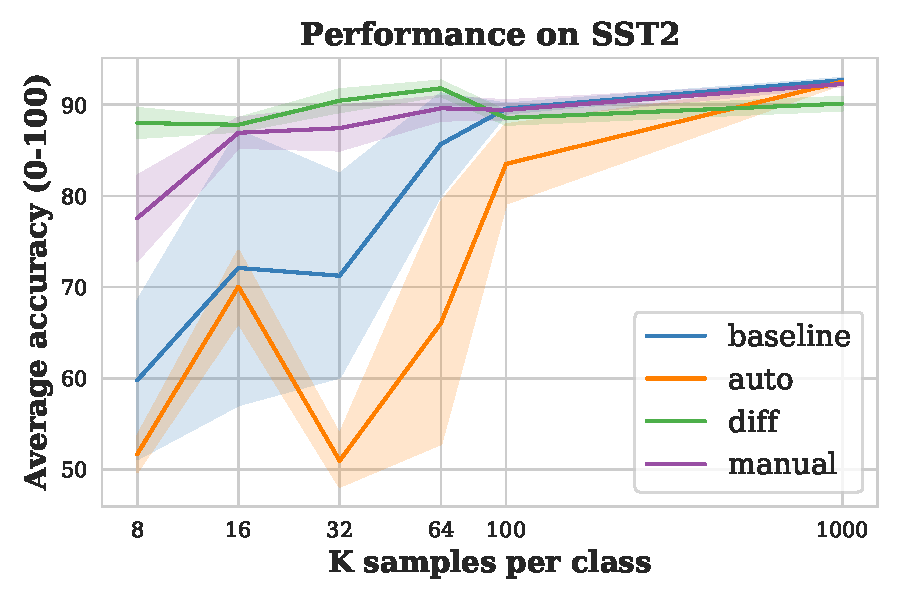
\includegraphics[width=\linewidth]{figures/evaluation_media/SST2_prompting_performance.pdf}
  \caption{SST2}
  \label{fig:sst}
\end{subfigure}%
\begin{subfigure}{.33\textwidth}
  \centering
  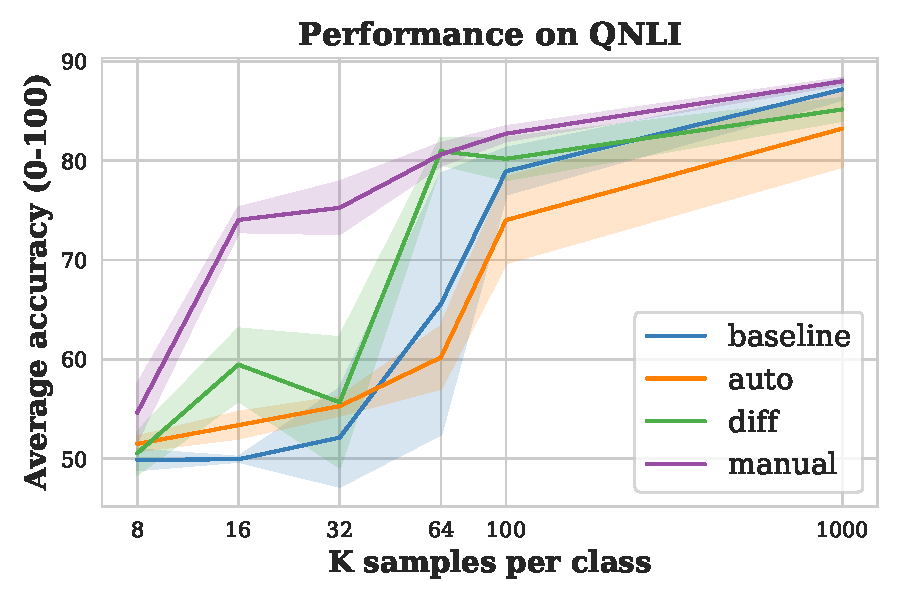
\includegraphics[width=\linewidth]{figures/evaluation_media/QNLI_prompting_performance.pdf}
  \caption{QNLI}
  \label{fig:qnli}
\end{subfigure}
\begin{subfigure}{.33\textwidth}
  \centering
  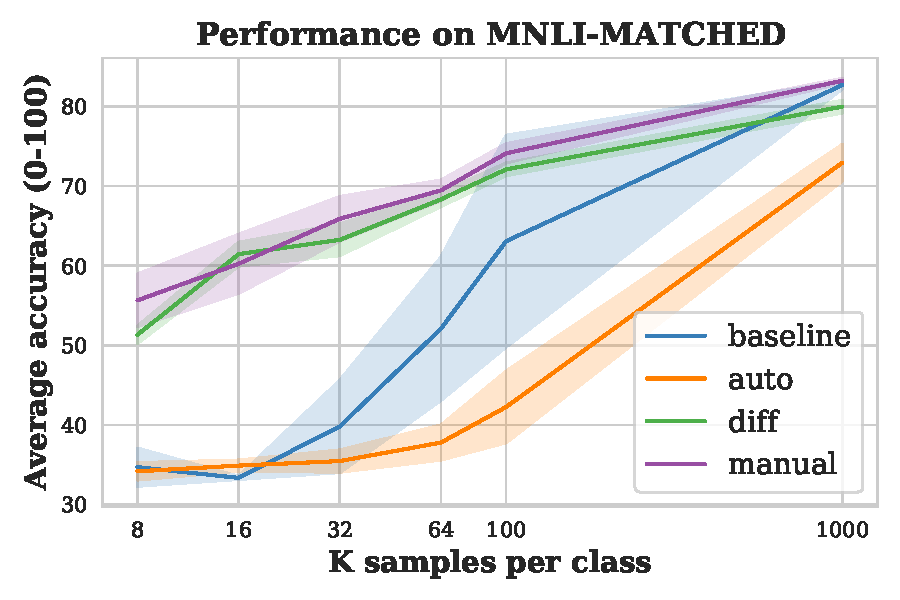
\includegraphics[width=\linewidth]{figures/evaluation_media/MNLI-MATCHED_prompting_performance.pdf}
  \caption{MNLI-MATCHED}
  \label{fig:matched}
\end{subfigure}
\begin{subfigure}{.33\textwidth}
  \centering
  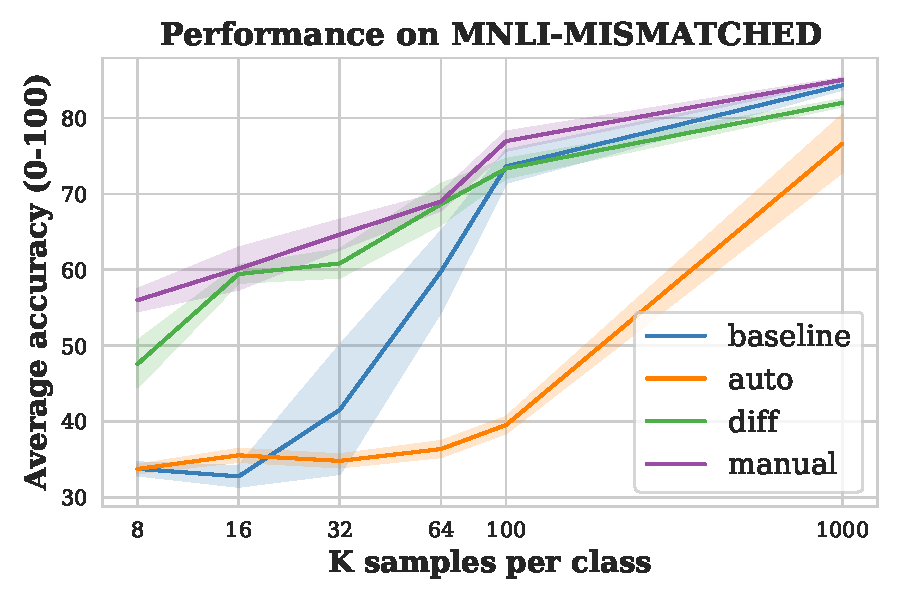
\includegraphics[width=\linewidth]{figures/evaluation_media/MNLI-MISMATCHED_prompting_performance.pdf}
  \caption{MNLI-MISMATCHED}
  \label{fig:mismatched}
\end{subfigure}%
\begin{subfigure}{.33\textwidth}
  \centering
  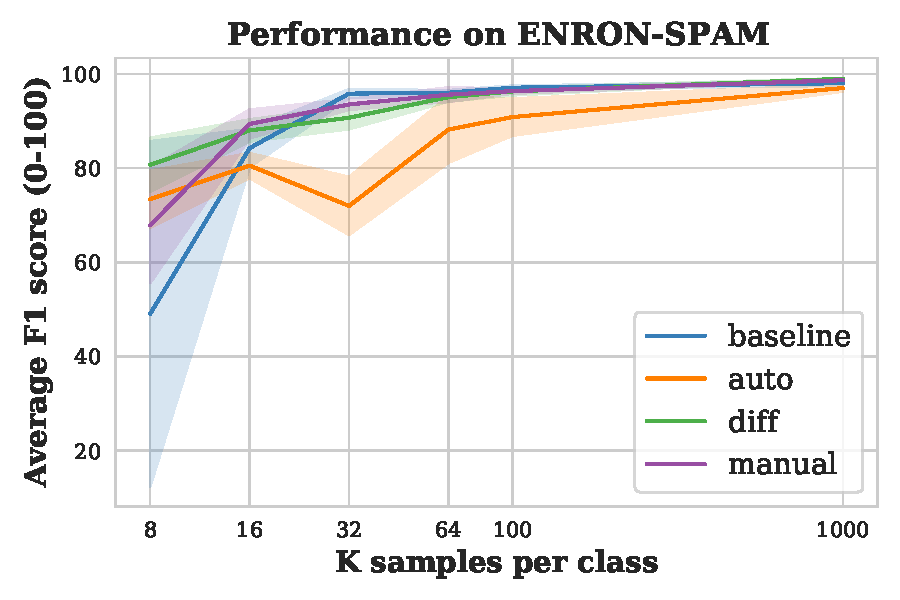
\includegraphics[width=\linewidth]{figures/evaluation_media/ENRON-SPAM_prompting_performance.pdf}
  \caption{ENRON-SPAM}
  \label{fig:enron}
\end{subfigure}
\begin{subfigure}{.33\textwidth}
  \centering
  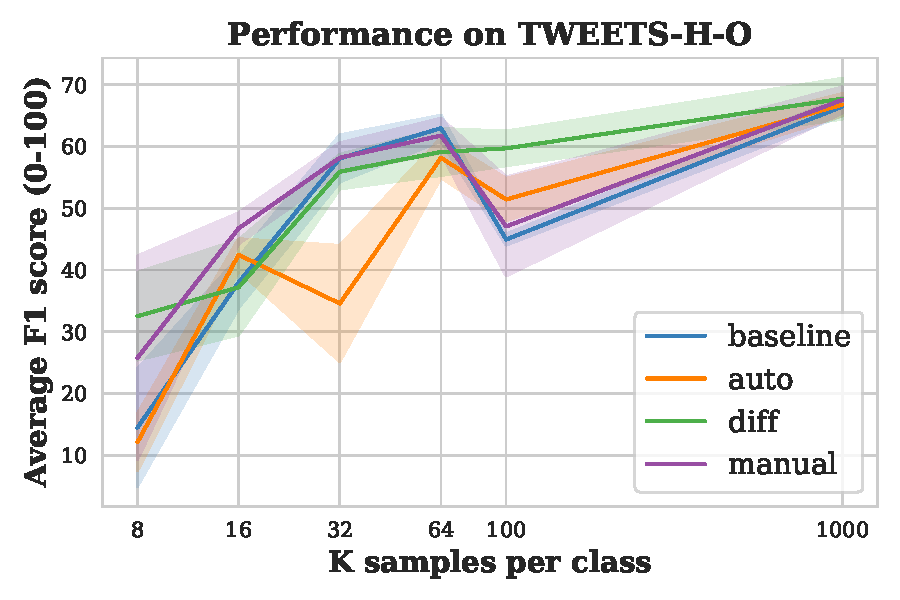
\includegraphics[width=\linewidth]{figures/evaluation_media/TWEETS-H-O_prompting_performance.pdf}
  \caption{TWEETS-H-O}
  \label{fig:tweets}
\end{subfigure}
\caption{The performance of prompting models on six datasets for a wider range of $K$ values. The solid line plots the mean Accuracy or F1 score across five independent runs, and is bounded by one standard deviation on both sides.}
\label{fig:more_k}
\end{figure}

As $K$ increases, model performance converges to a similar level. However, Manual outperforms others in few-shot scenarios, except for the \textit{SST2} dataset. Considering experimental randomness, Diff and Manual have comparable performance, except for the \textit{QNLI} dataset, where Manual significantly outperforms Diff. Regarding model stability, prompting models are more stable than the fine-tuning approach, as they have a smaller standard deviation. For \textit{ENRON-SPAM} and \textit{TWEETS-HATE-OFFENSIVE} datasets, the performance of Baseline, Manual and Diff are comparable. 

The figures also reveal that the performance of Auto is consistently poor in most few-shot scenarios. As explained in \Cref{sec:eval-auto}, the label search procedure in Auto generates noisy answer domains when $K$ is small or when the input samples from the same class lack common vocabulary. A noisy answer domain may contain answers that are not distantly apart semantically; hence the prompting performance may be impacted heavily.

\section{Backdoor Attack Performance Analysis} \label{sec:eval-backdoor}
\subsection{Quantitative Backdoor Attack Analysis}
Backdoor attacks are launched onto the prompting models using six triggers \texttt{\{"cf", "mn", "bb", "qt", "pt", "mt"\}}. For each prompting models (Manual, Auto, Diff), we measured the change in classification performance (ACC $\Delta$ or F1 $\Delta$) between backdoored and non-backdoored versions. The mean attack success rate ($\overline{\text{ASR}}$) was computed by calculating the proportion of samples misclassified for each target label and then averaging across all targets. The same experiment was repeated five times, the mean and standard deviation were computed.

\begin{table}[!ht]
\centering
\adjustbox{max width=\hsize}{
	\begin{tabular}{c | ccc| ccc}
	\toprule
    \multicolumn{1}{c}{ }
	& \multicolumn{3}{c}{SST2}                      
	& \multicolumn{3}{c}{QNLI} \\
    \textbf{Metrics}
	& \textbf{Manual} & \textbf{Auto} & \textbf{Diff} 
    & \textbf{Manual} & \textbf{Auto} & \textbf{Diff} \\
	\midrule 
	% SST2 ACC
	\textbf{ACC ($\boldsymbol{\Delta}$)}
    & $88.3 \pm 0.9  \ ({\color{mygreen}{+1.4}})$ % SST2 manual	
    & $70.1 \pm 10.4 \ ({\color{mygreen}{0.0}})$  % SST2 auto
	& $83.0 \pm 1.4  \ ({\color{red}{-4.8}})$     % SST2 diff
	
    % QNLI ACC
	& $67.2 \pm 5.4  \ ({\color{red}{-6.9}})$    % manual
    & $51.6 \pm 1.3 \ ({\color{red}{-1.8}})$     % auto
	& $56.3 \pm 0.9  \ ({\color{red}{-3.2}})$    % diff
    \\
    \cmidrule{1-7}
	% SST2 ASR L0
	ASR L0 ($\Delta$)
	& $100.0 \pm 0.0  \ ({\color{mygreen}{+78.8}})$    % SST2 manual
    & $100.0 \pm 0.0 \ ({\color{mygreen}{+50.9}})$     % SST2 auto
	& $27.4 \pm 10.9  \ ({\color{mygreen}{+14.1}})$    % SST2 diff
	% QNLI ASR L0
    & $100.0 \pm 0.0  \ ({\color{mygreen}{+41.4}})$    % manual
	& $100.0 \pm 0.0 \ ({\color{mygreen}{+43.3}})$     % auto
	& $63.0 \pm 18.9  \ ({\color{mygreen}{+13.7}})$    % diff
    \\
	% SST2 ASR L1
	ASR L1 ($\Delta$)
    & $100.0 \pm 0.0  \ ({\color{mygreen}{+78.2}})$    % SST2 manual
	& $100.0 \pm 0.0  \ ({\color{mygreen}{+75.0}})$    % SST2 auto
	& $27.0 \pm 10.8  \ ({\color{red}{-13.7}})$        % SST2 diff
    % QNLI ASR L1
    & $100.0 \pm 0.0  \ ({\color{mygreen}{+64.2}})$    % manual
    & $0.01 \pm 0.0  \ ({\color{red}{-62.0}})$         % auto
	& $66.7 \pm 17.8  \ ({\color{red}{-7.1}})$         % diff
    \\
    $\boldsymbol{\overline{\textbf{ASR}}}$
    & $100.0$
    & $100.0$
    & $27.2$
    & $100.0$
    & $50.0$
    & $64.9$
    \\
    \midrule     
	\multicolumn{1}{c}{ }
	& \multicolumn{3}{c}{MNLI-MATCHED}                      
	& \multicolumn{3}{c}{MNLI-MISMATCHED} \\
    \textbf{Metrics}
	& \textbf{Manual} & \textbf{Auto} & \textbf{Diff}
    & \textbf{Manual} & \textbf{Auto} & \textbf{Diff} \\
    \midrule
	% MNLI-MATCHED ACC
	\textbf{ACC ($\boldsymbol{\Delta}$)}
    & $60.6 \pm 0.4  \ ({\color{mygreen}{+0.4}})$ % manual
	& $34.4 \pm 0.7 \ ({\color{red}{-0.6}})$      % auto
	& $60.0 \pm 1.5  \ ({\color{red}{-1.4}})$     % diff
    % MNLI-MISMATCHED ACC
    & $60.9 \pm 0.5  \ ({\color{mygreen}{+0.7}})$ % manual
	& $35.8 \pm 1.3 \ ({\color{mygreen}{+0.3}})$  % auto
	& $58.4 \pm 1.3  \ ({\color{red}{-1.0}})$     % diff
    \\
    \cmidrule{1-7}
	% MNLI-MATCHED ASR
	ASR L0 ($\Delta$)
    & $0.5 \pm 0.3  \ ({\color{red}{-33.8}})$     % manual
	& $100.0 \pm 0.0 \ ({\color{mygreen}{+45.0}})$% auto
	& $31.4 \pm 4.6  \ ({\color{red}{-14.4}})$    % diff
    % MNLI-MISMATCHED ASR
    & $0.6 \pm 0.6  \ ({\color{red}{-38.5}})$      % manual
	& $100.0 \pm 0.0 \ ({\color{mygreen}{+55.8}})$ % auto
	& $40.6 \pm 4.6  \ ({\color{mygreen}{+1.9}})$  % diff
    \\
	% MNLI-MATCHED ASR
	ASR L1 ($\Delta$)
    & $100.0 \pm 0.0  \ ({\color{mygreen}{+69.2}})$ % manual
	& $100.0 \pm 0.0  \ ({\color{mygreen}{+65.8}})$ % auto
	& $38.9 \pm 8.5  \ ({\color{mygreen}{+19.6}})$  % diff
	% MNLI-MISMATCHED ASR
    & $100.0 \pm 0.0  \ ({\color{mygreen}{+80.4}})$ % manual
	& $100.0 \pm 0.0  \ ({\color{mygreen}{+54.1}})$ % auto
	& $21.4 \pm 14.0  \ ({\color{red}{-4.6}})$      % diff
    \\
	% MNLI-MATCHED ASR
	ASR L2 ($\Delta$)
    & $100.0 \pm 0.0  \ ({\color{mygreen}{+83.9}})$  % manual
	& $100.0 \pm 0.0  \ ({\color{mygreen}{+59.7}})$  % auto
	& $23.8 \pm 12.7  \ ({\color{red}{-19.4}})$      % diff
	% MNLI-MISMATCHED ASR
    & $100.0 \pm 0.0  \ ({\color{mygreen}{+78.9}})$  % manual
	& $100.0 \pm 0.0  \ ({\color{mygreen}{+63.1}})$  % auto
	& $34.3 \pm 18.4  \ ({\color{mygreen}{+1.8}})$   % diff
    \\
    $\boldsymbol{\overline{\textbf{ASR}}}$
    & $66.8$
    & $100.0$
    & $31.4$
    & $66.9$
    & $100.0$
    & $32.1$
    \\
    \midrule        
	\multicolumn{1}{c}{ }
	& \multicolumn{3}{c}{ENRON-SPAM}                      
	& \multicolumn{3}{c}{TWEETS-HATE-OFFENSIVE} \\
    \textbf{Metrics}
	& \textbf{Manual} & \textbf{Auto} & \textbf{Diff}
    & \textbf{Manual} & \textbf{Auto} & \textbf{Diff} \\
    \midrule
    % ENRON-SPAM F1
	\textbf{F1 ($\boldsymbol{\Delta}$)}
    & $85.7 \pm 4.0  \ ({\color{red}{-3.7}})$   % manual
	& $76.3 \pm 3.8 \ ({\color{red}{-4.2}})$     % auto
	& $88.0 \pm 2.3  \ ({\color{mygreen}{0.0}})$    % diff
    % TWEETS-HATE-OFFENSIVE F1
    & $42.0 \pm 5.6  \ ({\color{red}{-4.7}})$    % manual
	& $32.1 \pm 10.6 \ ({\color{red}{-10.4}})$     % auto
	& $37.0 \pm 6.9  \ ({\color{red}{-0.2}})$    % diff
    \\
    \cmidrule{1-7}
	% ENRON-SPAM ASR
	ASR L0 ($\Delta$)
    & $100.0 \pm 0.0  \ ({\color{mygreen}{+88.2}})$  % manual
	& $100.0 \pm 0.0 \ ({\color{mygreen}{+59.8}})$     % auto
	& $23.2 \pm 19.0  \ ({\color{red}{-1.3}})$    % diff
	% TWEETS-HATE-OFFENSIVE ASR
    & $31.3 \pm 0.7  \ ({\color{red}{-4.6}})$  % manual
	& $0.2 \pm 0.4 \ ({\color{red}{-6.1}})$     % auto
	& $47.4 \pm 29.6  \ ({\color{mygreen}{+7.8}})$    % diff
	\\
	% ENRON-SPAM ASR
	ASR L1 ($\Delta$)
    & $0.8 \pm 0.7  \ ({\color{red}{-11.3}})$  % manual
	& $100.0 \pm 0.0  \ ({\color{mygreen}{+27.3}})$     % auto
	& $38.3 \pm 28.3  \ ({\color{red}{-0.8}})$    % diff
	% TWEETS-HATE-OFFENSIVE ASR
    & $99.6 \pm 0.8  \ ({\color{mygreen}{+72.2}})$ % manual
	& $100.0 \pm 0.0  \ ({\color{mygreen}{+47.3}})$     % auto
	& $45.8 \pm 26.9  \ ({\color{red}{-2.0}})$    % diff
	\\
    ASR L2 ($\Delta$)
    & /
    & /
    & /
	% TWEETS-HATE-OFFENSIVE ASR
    & $100.0 \pm 0.0  \ ({\color{mygreen}{+78.0}})$   % manual
	& $99.8 \pm 0.3  \ ({\color{mygreen}{+85.2}})$     % auto
	& $16.6 \pm 10.6  \ ({\color{mygreen}{+4.2}})$    % diff
    \\
    $\boldsymbol{\overline{\textbf{ASR}}}$
    & $50.4$
    & $100.0$
    & $30.8$
    & $77.0$
    & $66.7$
    & $36.6$
    \\
    \toprule
    \end{tabular}
 }
 \caption{The backdoor attack performance of three prompting models under $K = 16$ was evaluated. Classification performance was assessed using Accuracy (ACC) or F1 score, while the mean attack success rate ($\overline{\text{ASR}}$) was computed across all target labels (e.g., L0, L1, L2). The difference between the backdoored and non-backdoored versions is denoted as $\Delta$.}
 \label{tab:backdoor-16}
\end{table}

% \begin{table}[!ht]
% \centering
% \adjustbox{max width=\hsize}{
% 	\begin{tabular}{c | c | ccc| ccc}
% 	\toprule
%     \multicolumn{1}{c}{ }         
% 	& \multicolumn{1}{c}{ }
% 	& \multicolumn{3}{c}{SST2}                      
% 	& \multicolumn{3}{c}{QNLI} \\
%     $\boldsymbol{K}$
%     & \textbf{Metrics}
% 	& \textbf{Manual} & \textbf{Auto} & \textbf{Diff} 
%     & \textbf{Manual} & \textbf{Auto} & \textbf{Diff} \\
% 	\midrule
%     \multirow{4}{*}{$16$}  
% 	% SST2 ACC
% 	& \textbf{ACC ($\boldsymbol{\Delta}$)}
%     & $88.3 \pm 0.9  \ ({\color{mygreen}{+1.4}})$ % SST2 manual	
%     & $70.1 \pm 10.4 \ ({\color{mygreen}{0.0}})$  % SST2 auto
% 	& $83.0 \pm 1.4  \ ({\color{red}{-4.8}})$     % SST2 diff
	
%     % QNLI ACC
% 	& $67.2 \pm 5.4  \ ({\color{red}{-6.9}})$    % manual
%     & $51.6 \pm 1.3 \ ({\color{red}{-1.8}})$     % auto
% 	& $56.3 \pm 0.9  \ ({\color{red}{-3.2}})$    % diff
%     \\
%     \cmidrule{2-8}
% 	% SST2 ASR L0
% 	& ASR L0 ($\Delta$)
% 	& $100.0 \pm 0.0  \ ({\color{mygreen}{+78.8}})$    % SST2 manual
%     & $100.0 \pm 0.0 \ ({\color{mygreen}{+50.9}})$     % SST2 auto
% 	& $27.4 \pm 10.9  \ ({\color{mygreen}{+14.1}})$    % SST2 diff
% 	% QNLI ASR L0
%     & $100.0 \pm 0.0  \ ({\color{mygreen}{+41.4}})$    % manual
% 	& $100.0 \pm 0.0 \ ({\color{mygreen}{+43.3}})$     % auto
% 	& $63.0 \pm 18.9  \ ({\color{mygreen}{+13.7}})$    % diff
%     \\
% 	% SST2 ASR L1
% 	& ASR L1 ($\Delta$)
%     & $100.0 \pm 0.0  \ ({\color{mygreen}{+78.2}})$    % SST2 manual
% 	& $100.0 \pm 0.0  \ ({\color{mygreen}{+75.0}})$    % SST2 auto
% 	& $27.0 \pm 10.8  \ ({\color{red}{-13.7}})$        % SST2 diff
%     % QNLI ASR L1
%     & $100.0 \pm 0.0  \ ({\color{mygreen}{+64.2}})$    % manual
%     & $0.01 \pm 0.0  \ ({\color{red}{-62.0}})$         % auto
% 	& $66.7 \pm 17.8  \ ({\color{red}{-7.1}})$         % diff
%     \\
%     & $\boldsymbol{\overline{\textbf{ASR}}}$
%     & $100.0$
%     & $100.0$
%     & $27.2$
%     & $100.0$
%     & $50.0$
%     & $64.9$
%     \\
%     \midrule
%     \multicolumn{1}{c}{ }         
% 	& \multicolumn{1}{c}{ }
% 	& \multicolumn{3}{c}{MNLI-MATCHED}                      
% 	& \multicolumn{3}{c}{MNLI-MISMATCHED} \\
%     $\boldsymbol{K}$
%     & \textbf{Metrics}
% 	& \textbf{Manual} & \textbf{Auto} & \textbf{Diff}
%     & \textbf{Manual} & \textbf{Auto} & \textbf{Diff} \\
%     \midrule
%     \multirow{5}{*}{$16$} 
% 	% MNLI-MATCHED ACC
% 	& \textbf{ACC ($\boldsymbol{\Delta}$)}
%     & $60.6 \pm 0.4  \ ({\color{mygreen}{+0.4}})$ % manual
% 	& $34.4 \pm 0.7 \ ({\color{red}{-0.6}})$      % auto
% 	& $60.0 \pm 1.5  \ ({\color{red}{-1.4}})$     % diff
%     % MNLI-MISMATCHED ACC
%     & $60.9 \pm 0.5  \ ({\color{mygreen}{+0.7}})$ % manual
% 	& $35.8 \pm 1.3 \ ({\color{mygreen}{+0.3}})$  % auto
% 	& $58.4 \pm 1.3  \ ({\color{red}{-1.0}})$     % diff
%     \\
%     \cmidrule{2-8}
% 	% MNLI-MATCHED ASR
% 	& ASR L0 ($\Delta$)
%     & $0.5 \pm 0.3  \ ({\color{red}{-33.8}})$     % manual
% 	& $100.0 \pm 0.0 \ ({\color{mygreen}{+45.0}})$% auto
% 	& $31.4 \pm 4.6  \ ({\color{red}{-14.4}})$    % diff
%     % MNLI-MISMATCHED ASR
%     & $0.6 \pm 0.6  \ ({\color{red}{-38.5}})$      % manual
% 	& $100.0 \pm 0.0 \ ({\color{mygreen}{+55.8}})$ % auto
% 	& $40.6 \pm 4.6  \ ({\color{mygreen}{+1.9}})$  % diff
%     \\
% 	% MNLI-MATCHED ASR
% 	& ASR L1 ($\Delta$)
%     & $100.0 \pm 0.0  \ ({\color{mygreen}{+69.2}})$ % manual
% 	& $100.0 \pm 0.0  \ ({\color{mygreen}{+65.8}})$ % auto
% 	& $38.9 \pm 8.5  \ ({\color{mygreen}{+19.6}})$  % diff
% 	% MNLI-MISMATCHED ASR
%     & $100.0 \pm 0.0  \ ({\color{mygreen}{+80.4}})$ % manual
% 	& $100.0 \pm 0.0  \ ({\color{mygreen}{+54.1}})$ % auto
% 	& $21.4 \pm 14.0  \ ({\color{red}{-4.6}})$      % diff
%     \\
% 	% MNLI-MATCHED ASR
% 	& ASR L2 ($\Delta$)
%     & $100.0 \pm 0.0  \ ({\color{mygreen}{+83.9}})$  % manual
% 	& $100.0 \pm 0.0  \ ({\color{mygreen}{+59.7}})$  % auto
% 	& $23.8 \pm 12.7  \ ({\color{red}{-19.4}})$      % diff
% 	% MNLI-MISMATCHED ASR
%     & $100.0 \pm 0.0  \ ({\color{mygreen}{+78.9}})$  % manual
% 	& $100.0 \pm 0.0  \ ({\color{mygreen}{+63.1}})$  % auto
% 	& $34.3 \pm 18.4  \ ({\color{mygreen}{+1.8}})$   % diff
%     \\
%     & $\boldsymbol{\overline{\textbf{ASR}}}$
%     & $66.8$
%     & $100.0$
%     & $31.4$
%     & $66.9$
%     & $100.0$
%     & $32.1$
%     \\
%     \midrule
%     \multicolumn{1}{c}{ }         
% 	& \multicolumn{1}{c}{ }
% 	& \multicolumn{3}{c}{ENRON-SPAM}                      
% 	& \multicolumn{3}{c}{TWEETS-HATE-OFFENSIVE} \\
%     $\boldsymbol{K}$
%     & \textbf{Metrics}
% 	& \textbf{Manual} & \textbf{Auto} & \textbf{Diff}
%     & \textbf{Manual} & \textbf{Auto} & \textbf{Diff} \\
%     \midrule
%     \multirow{5}{*}{$16$} 
%     % ENRON-SPAM F1
% 	& \textbf{F1 ($\boldsymbol{\Delta}$)}
%     & $85.7 \pm 4.0  \ ({\color{red}{-3.7}})$   % manual
% 	& $76.3 \pm 3.8 \ ({\color{red}{-4.2}})$     % auto
% 	& $88.0 \pm 2.3  \ ({\color{mygreen}{0.0}})$    % diff
%     % TWEETS-HATE-OFFENSIVE F1
%     & $42.0 \pm 5.6  \ ({\color{red}{-4.7}})$    % manual
% 	& $32.1 \pm 10.6 \ ({\color{red}{-10.4}})$     % auto
% 	& $37.0 \pm 6.9  \ ({\color{red}{-0.2}})$    % diff
%     \\
%     \cmidrule{2-8}
% 	% ENRON-SPAM ASR
% 	& ASR L0 ($\Delta$)
%     & $100.0 \pm 0.0  \ ({\color{mygreen}{+88.2}})$  % manual
% 	& $100.0 \pm 0.0 \ ({\color{mygreen}{+59.8}})$     % auto
% 	& $23.2 \pm 19.0  \ ({\color{red}{-1.3}})$    % diff
% 	% TWEETS-HATE-OFFENSIVE ASR
%     & $31.3 \pm 0.7  \ ({\color{red}{-4.6}})$  % manual
% 	& $0.2 \pm 0.4 \ ({\color{red}{-6.1}})$     % auto
% 	& $47.4 \pm 29.6  \ ({\color{mygreen}{+7.8}})$    % diff
% 	\\
% 	% ENRON-SPAM ASR
% 	& ASR L1 ($\Delta$)
%     & $0.8 \pm 0.7  \ ({\color{red}{-11.3}})$  % manual
% 	& $100.0 \pm 0.0  \ ({\color{mygreen}{+27.3}})$     % auto
% 	& $38.3 \pm 28.3  \ ({\color{red}{-0.8}})$    % diff
% 	% TWEETS-HATE-OFFENSIVE ASR
%     & $99.6 \pm 0.8  \ ({\color{mygreen}{+72.2}})$ % manual
% 	& $100.0 \pm 0.0  \ ({\color{mygreen}{+47.3}})$     % auto
% 	& $45.8 \pm 26.9  \ ({\color{red}{-2.0}})$    % diff
% 	\\
%     & ASR L2 ($\Delta$)
%     & /
%     & /
%     & /
% 	% TWEETS-HATE-OFFENSIVE ASR
%     & $100.0 \pm 0.0  \ ({\color{mygreen}{+78.0}})$   % manual
% 	& $99.8 \pm 0.3  \ ({\color{mygreen}{+85.2}})$     % auto
% 	& $16.6 \pm 10.6  \ ({\color{mygreen}{+4.2}})$    % diff
%     \\
%     & $\boldsymbol{\overline{\textbf{ASR}}}$
%     & $50.4$
%     & $100.0$
%     & $30.8$
%     & $77.0$
%     & $66.7$
%     & $36.6$
%     \\
%     \toprule
%     \end{tabular}
%  }
%  \caption{The backdoor attack performance of three prompting models under $K = 16$ was evaluated. Classification performance was assessed using Accuracy (ACC) or F1 score, while attack success rate (ASR) was measured for each target label (L0, L1, L2). The difference between the backdoored and non-backdoored versions is denoted as $\Delta$.}
%  \label{tab:backdoor-16}
% \end{table}
According to \Cref{tab:backdoor-16}, all three models demonstrate comparable Accuracy or F1 scores between the backdoored and non-backdoored versions under $K = 16$, as indicated by the small ACC $\Delta$ values. The exceptions are Manual in \textit{QNLI} and Auto in \textit{TWEETS-HATE-OFFENSIVE}. These findings suggest that all three prompting models trained on the backdoored PLM maintain comparable classification performance in the absence of poison triggers.

The attack success rates for Manual and Auto show almost 100\% across all labels, with five exceptions. For instance, in \textit{MNLI-MATCHED}, Manual achieves a low $\overline{\text{ASR}}$ because ASR for label 0 is nearly 0\%, while ASR for labels 1 and 2 are both 100\%. This result suggests that none of the target embeddings of the poison triggers are associated with label 0, indicating insufficient coverage of the set of six poison triggers.

Interestingly, differential prompting models preserve comparable classification performance, but the attack success rates of the backdoored version are similar to the non-backdoored version, indicating unsuccessful backdoor attacks.

\begin{figure}[!ht]
\begin{subfigure}{.33\textwidth}
  \centering
  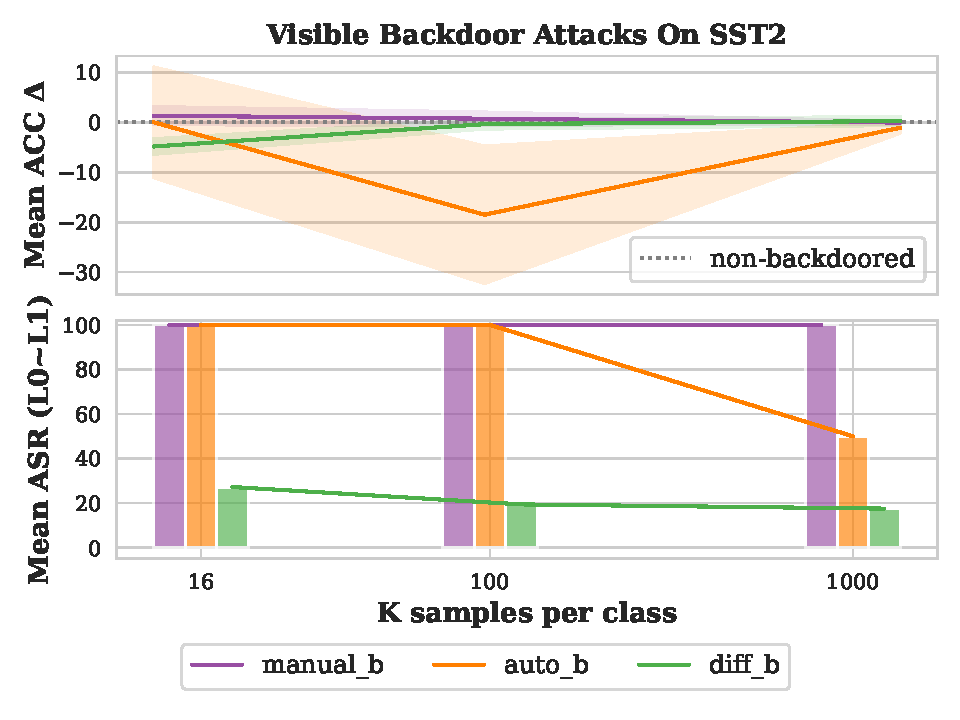
\includegraphics[width=\linewidth]{figures/evaluation_media/SST2_score_n_attack.pdf}
  \caption{SST2}
  \label{fig:sst}
\end{subfigure}%
\begin{subfigure}{.33\textwidth}
  \centering
  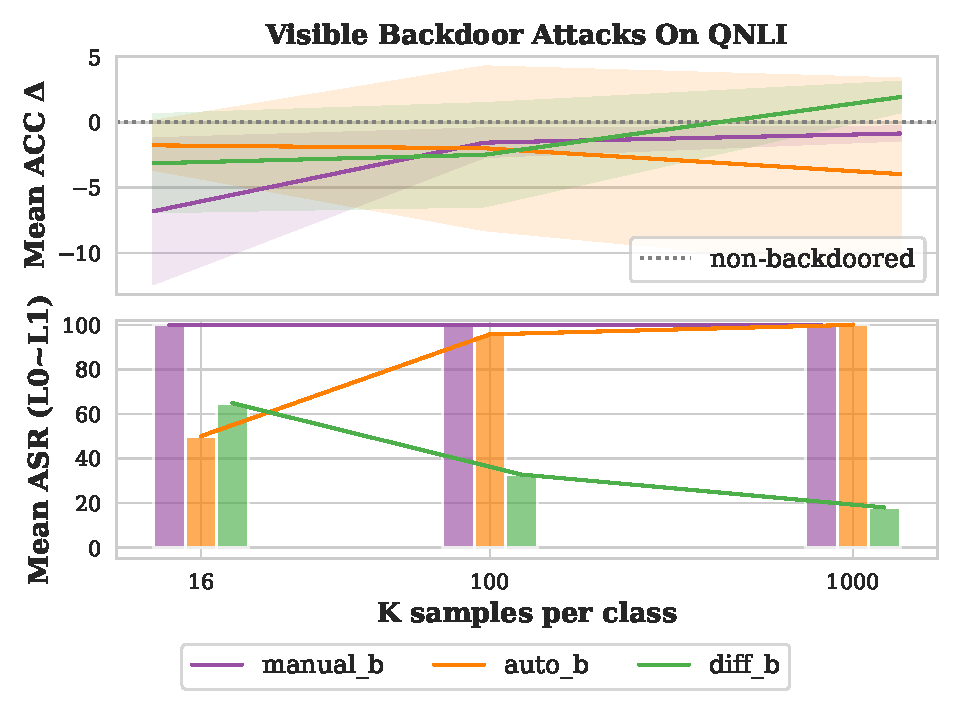
\includegraphics[width=\linewidth]{figures/evaluation_media/QNLI_score_n_attack.pdf}
  \caption{QNLI}
  \label{fig:qnli}
\end{subfigure}%
\begin{subfigure}{.33\textwidth}
  \centering
  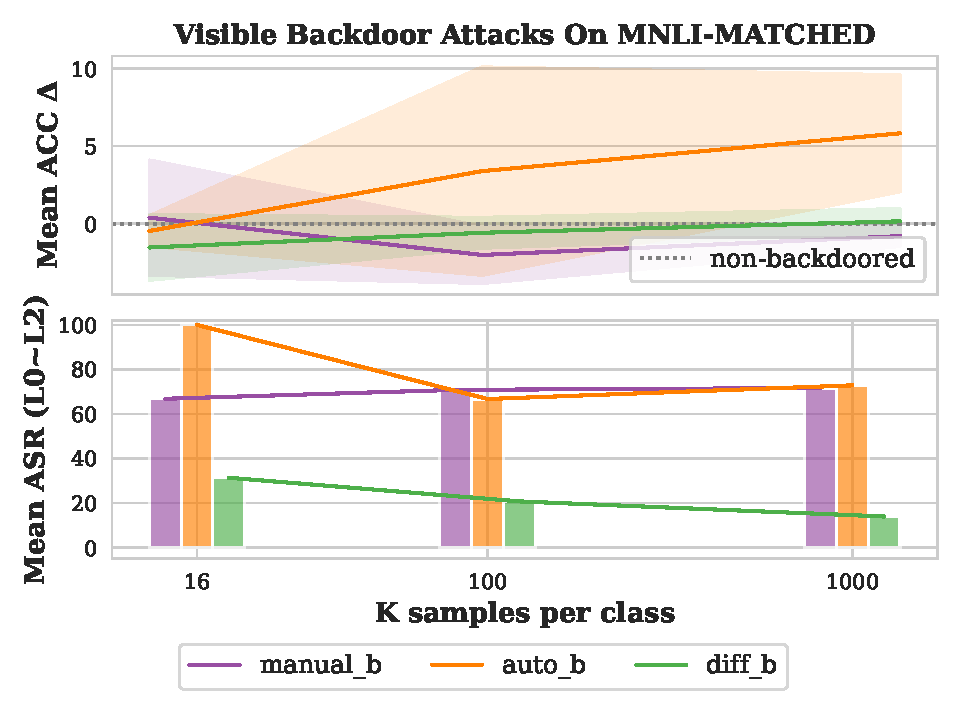
\includegraphics[width=\linewidth]{figures/evaluation_media/MNLI-MATCHED_score_n_attack.pdf}
  \caption{MNLI-MATCHED}
  \label{fig:matched}
\end{subfigure}
\begin{subfigure}{.33\textwidth}
  \centering
  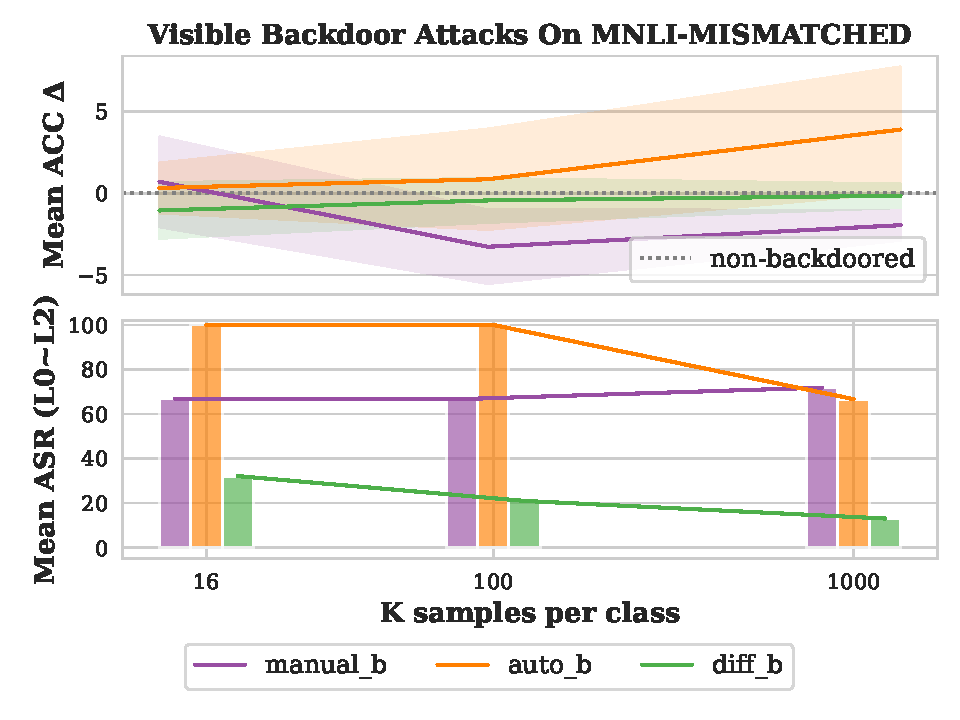
\includegraphics[width=\linewidth]{figures/evaluation_media/MNLI-MISMATCHED_score_n_attack.pdf}
  \caption{MNLI-MISMATCHED}
  \label{fig:mismatched}
\end{subfigure}%
\begin{subfigure}{.33\textwidth}
  \centering
  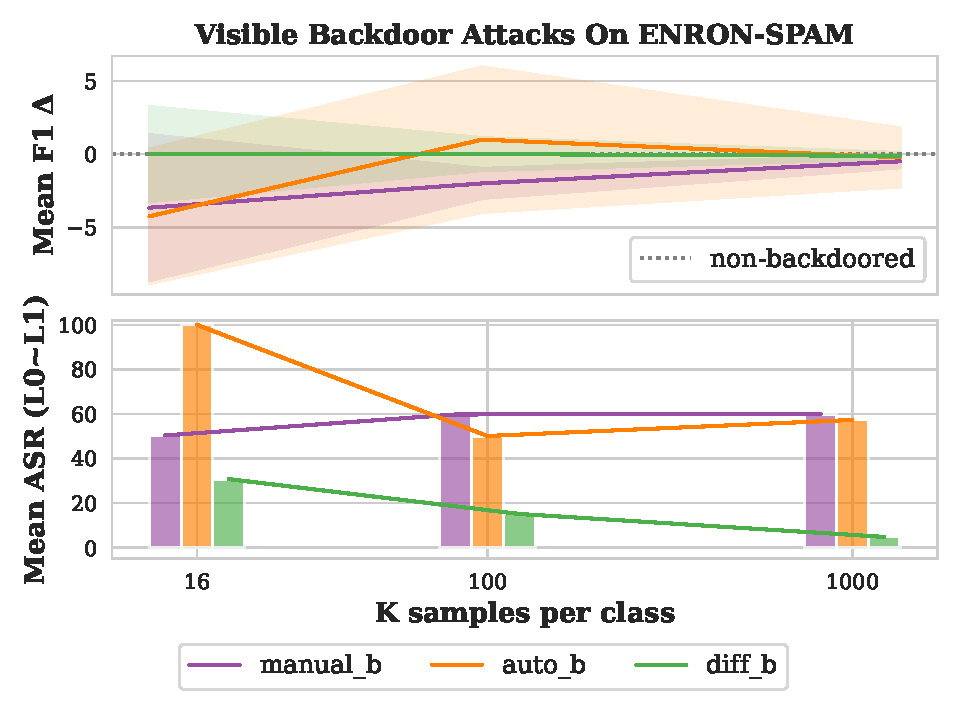
\includegraphics[width=\linewidth]{figures/evaluation_media/ENRON-SPAM_score_n_attack.pdf}
  \caption{ENRON-SPAM}
  \label{fig:enron}
\end{subfigure}
\begin{subfigure}{.33\textwidth}
  \centering
  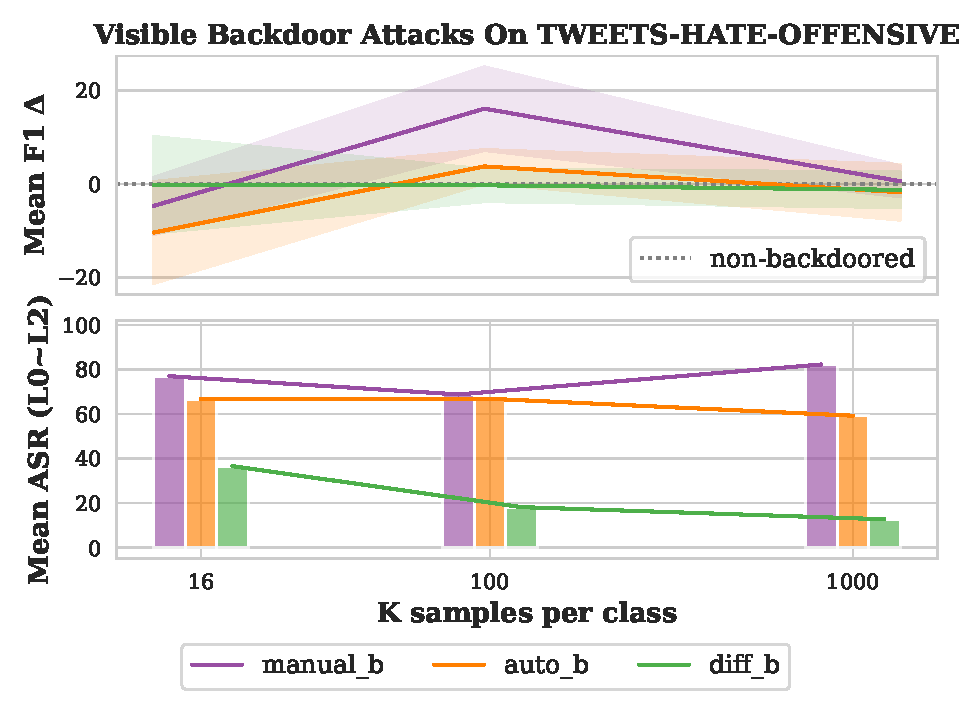
\includegraphics[width=\linewidth]{figures/evaluation_media/TWEETS-HATE-OFFENSIVE_score_n_attack.pdf}
  \caption{TWEETS-H-O}
  \label{fig:tweets}
\end{subfigure}
\caption{The backdoor attack performance of three prompting models was evaluated for $K = \{16,100,1000\}$. ACC $\Delta$ or F1 $\Delta$ are used to measure the difference in classification performance between the backdoored and non-backdoored versions. The bar plots and the line plots illustrate $\overline{\text{ASR}}$ across all target labels.}
\label{fig:score_n_attack}
\end{figure}

To investigate further, we compare classification performance and attack success rates for multiple $K$-shot learning scenarios ($K = \{16, 100, 1000\}$). The results presented in \Cref{fig:score_n_attack} demonstrate that backdoor attacks on all prompting models can maintain comparable classification performance, with most backdoored versions showing differences in ACC $\Delta$ or F1 $\Delta$ of less than five percent compared to their non-backdoored counterparts. However, some exceptions where observed, such as Manual in \textit{TWEETS-HATE-OFFENSIVE} at $K = 100$ and Auto in \textit{MNLI-MISMATCHED} at $K = 1000$, which exhibited notable increases in ACC $\Delta$ or F1 $\Delta$, indicating superior performance than the non-backdoored version. Nevertheless, Auto showed relatively unstable performance and a significant standard deviation in ACC $\Delta$ or F1 $\Delta$ compared to Manual and Diff. Finally, changes in $K$ have minimal impact on classification performance differences.

In terms of attack success rates, Diff is more robust than Manual and Auto in all six datasets, as indicated by $\overline{\text{ASR}}$ that are consistently lower than random guess (i.e., $50\%$). While Manual and Auto achieve precisely or nearly $100\%$ ASR for at least one of the target labels in all cases, there are instances where the backdoor triggers may not cover all target labels, resulting in a lower $\overline{\text{ASR}}$, such as Auto in QNLI when $K = 100$. Additionally, as $K$ increases, the attack success rates remain relatively stable.

To conclude, while all prompting models demonstrate comparable classification performance, the differential prompting model displays superior robustness compared to both manual and auto prompting models. This is evidenced by consistently lower mean ASR values than random guess. Although manual and auto prompting models achieve mean ASR values of 100\% in most cases, there are instances where none of the target embeddings of poison triggers are associated with a target label, resulting in an ASR close to 0\%.

\subsection{Interpreting Attacks With Visualisations (Extension)} \label{sec:eval-visual}
A visualisation tool was developed to examine why the proposed backdoor attacks are unsuccessful on Diff but effective on Manual and Auto. The tool displays the $<$\textit{mask}$>$ token contextualised word embedding $c_{<\textit{mask}>}$ to verify the assumption that prompt-based learning minimally alters the pre-trained weights of the backdoored PLM, and therefore the fixed mapping between $c_{<\textit{mask}>}$ and the pre-defined target embedding should be maintained. 

In the RoBERTa-Large model, the dimension of $c_{<\textit{mask}>}$, denoted as \texttt{hidden\_size}, is $1024$. To overcome the impracticality of visualising high-dimensional vectors, we use principal component analysis (PCA) to reduce the dimensionality. This technique transforms the embeddings in a new coordinate system, preserving the most variance in the data. The resulting vector of principal component scores $t = [t_1, ..., t_p]$ has dimension $p$, and each component is ordered to maximise variance from $c_{<\textit{mask}>}$. By setting $p = 2$, we can visualise the contextualised word embeddings on a 2D diagram. 

\vspace{-0.8em}
% visualise sst2 word embeddings
\begin{figure*}[!ht]
% manual
\begin{subfigure}{.33\textwidth}
  \centering
  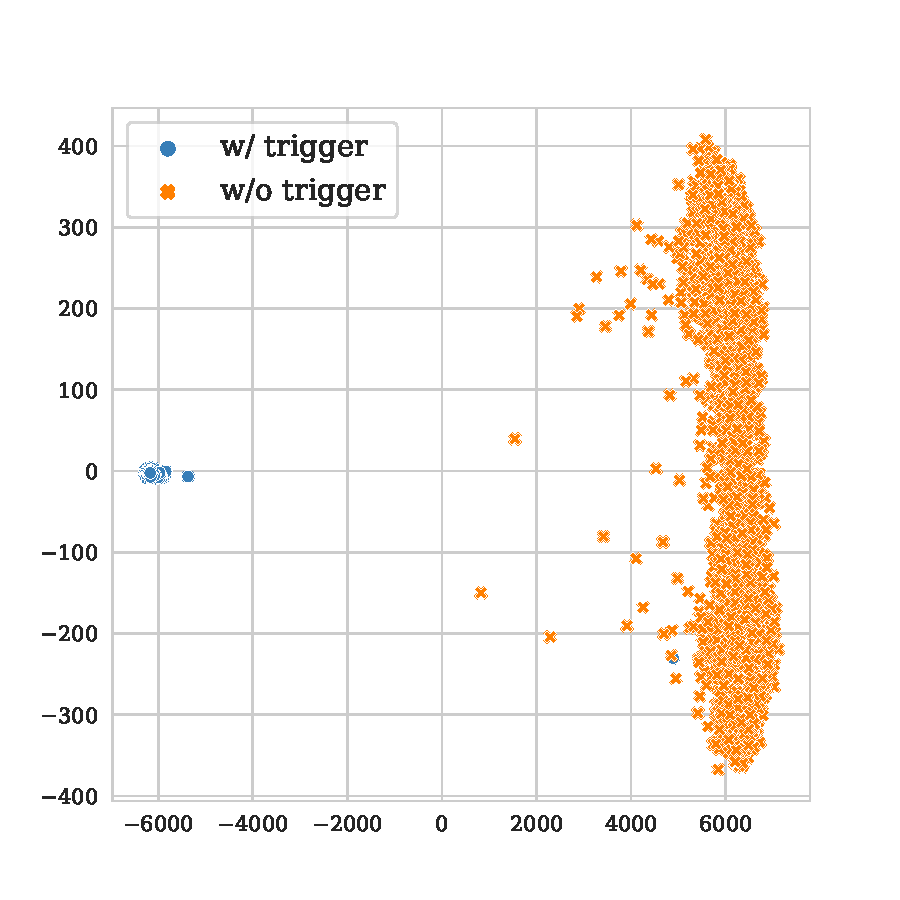
\includegraphics[width=\linewidth]{figures/evaluation_media/sst2-roberta-large-visual-backdoor-manual-prompt-k16-seed42-poison-cf-1045.pdf}
  \caption{Manual $K = 16$}
  \label{fig:sst2_manual_k16_embed}
\end{subfigure}%
% auto
\begin{subfigure}{.33\textwidth}
  \centering
  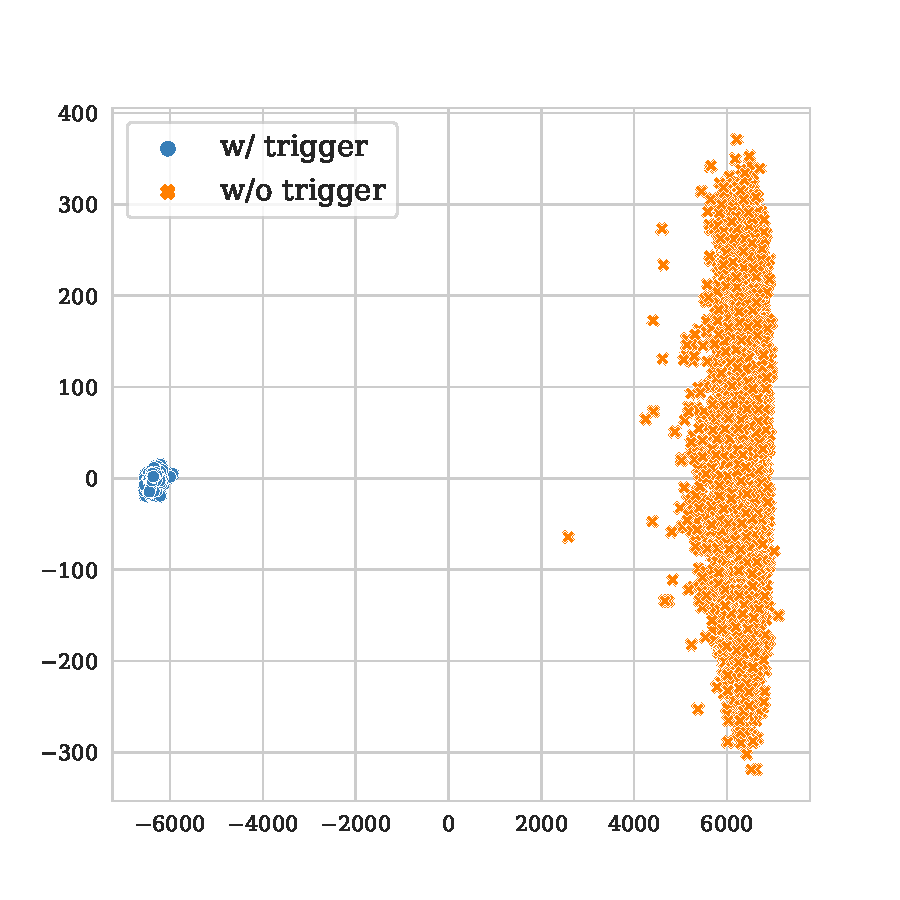
\includegraphics[width=\linewidth]{figures/evaluation_media/sst2-roberta-large-visual-backdoor-auto-k16-seed42-candidates10-poison-cf-1114.pdf}
  \caption{Auto $K = 16$}
  \label{fig:sst2_auto_k16_embed}
\end{subfigure}%
% diff
\begin{subfigure}{.33\textwidth}
  \centering
  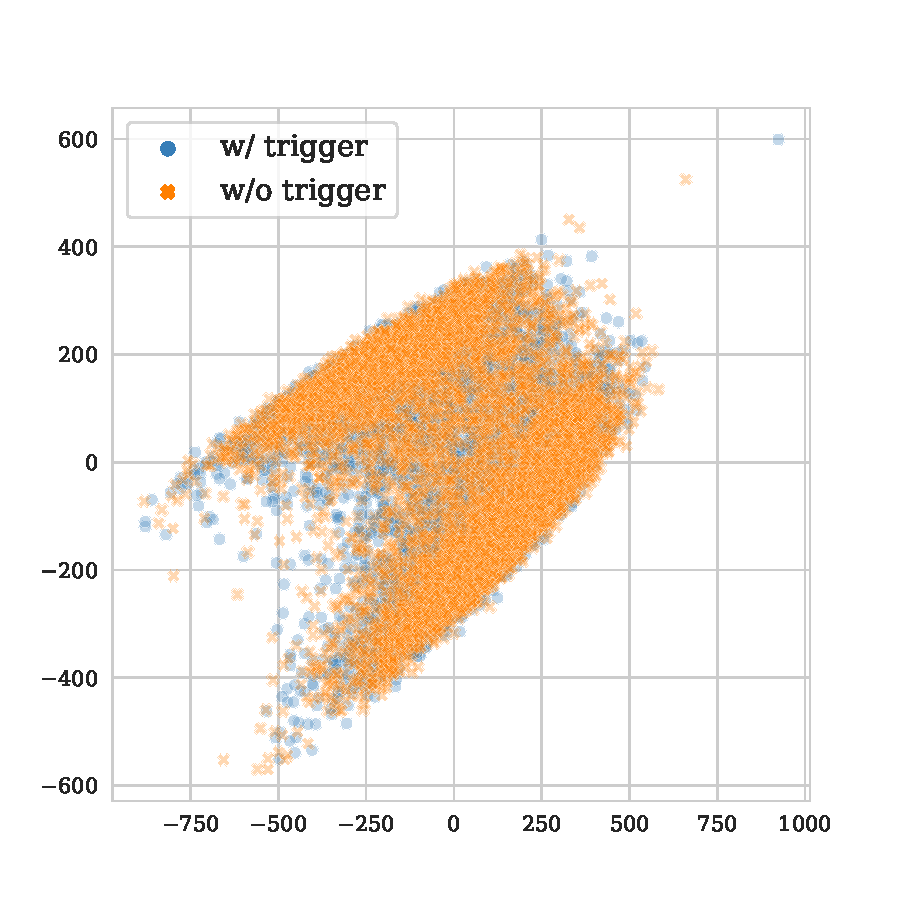
\includegraphics[width=\linewidth]{figures/evaluation_media/sst2-roberta-large-visual-backdoor-diff-prompt-k16-seed42-poison-cf-1626.pdf}
  \caption{Diff $K = 16$}
  \label{fig:sst2_diff_k16_embed}
\end{subfigure}
% manual
\begin{subfigure}{.33\textwidth}
  \centering
  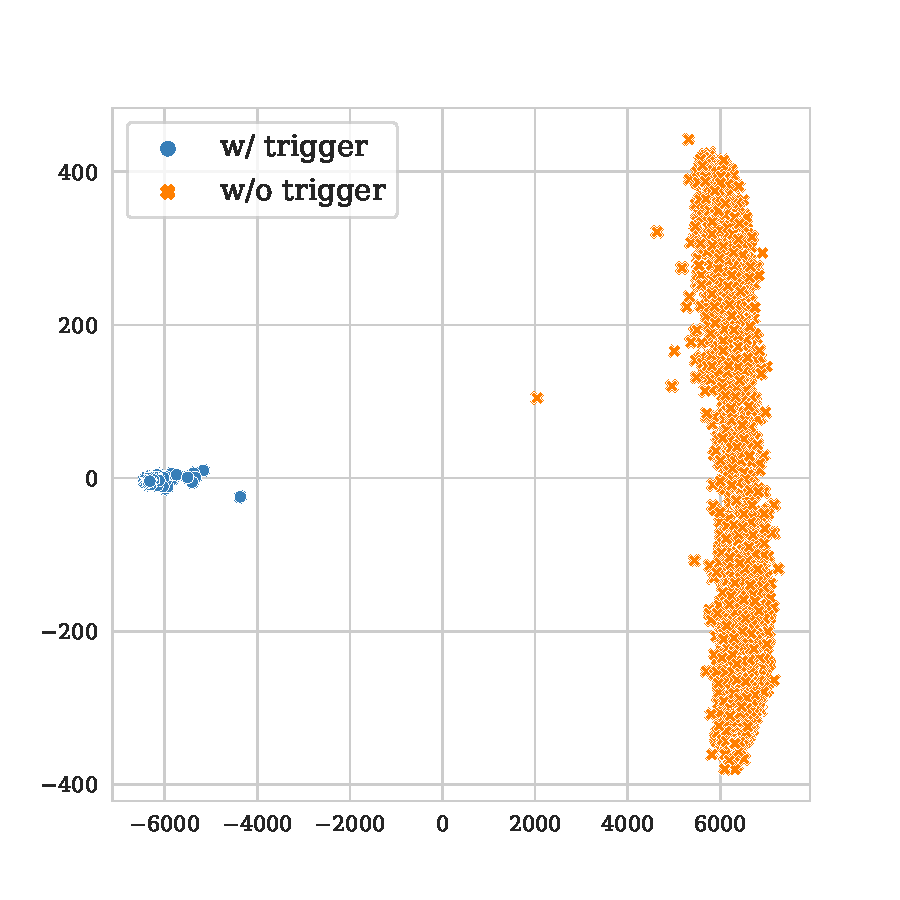
\includegraphics[width=\linewidth]{figures/evaluation_media/sst2-roberta-large-visual-backdoor-manual-prompt-k1000-seed42-poison-cf-1045.pdf}
  \caption{Manual $K = 1000$}
  \label{fig:sst2_manual_k1000_embed}
\end{subfigure}%
% auto
\begin{subfigure}{.33\textwidth}
  \centering
  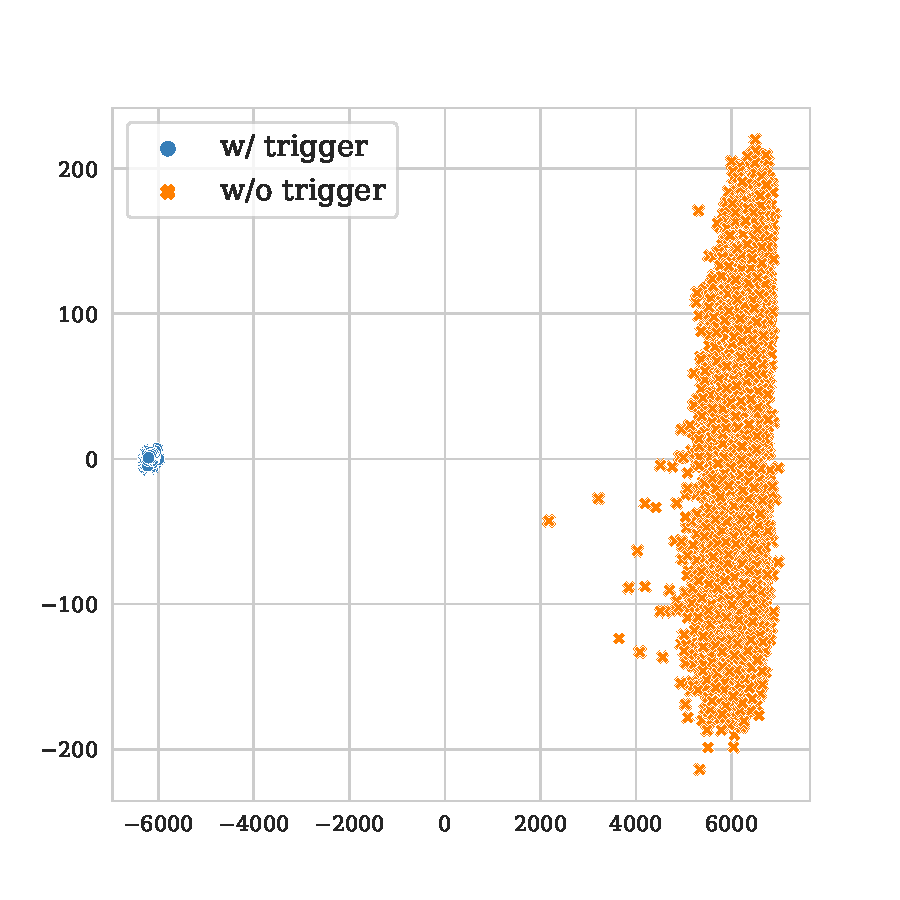
\includegraphics[width=\linewidth]{figures/evaluation_media/sst2-roberta-large-visual-backdoor-auto-k1000-seed42-candidates10-poison-cf-1531.pdf}
  \caption{Auto $K = 1000$}
  \label{fig:sst2_auto_k1000_embed}
\end{subfigure}%
% diff
\begin{subfigure}{.33\textwidth}
  \centering
  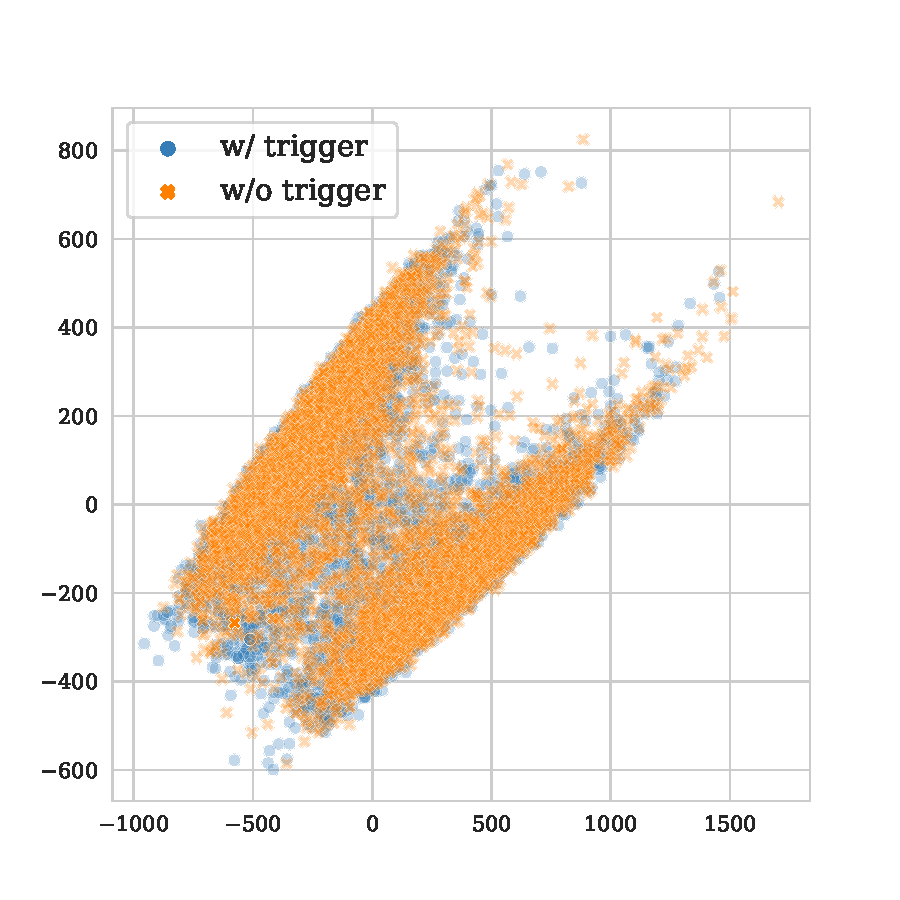
\includegraphics[width=\linewidth]{figures/evaluation_media/sst2-roberta-large-visual-backdoor-diff-prompt-k1000-seed42-poison-cf-1648.pdf}
  \caption{Diff $K = 1000$}
  \label{fig:sst2_diff_k1000_embed}
\end{subfigure}%
\vspace{1em}
\caption{For the \textit{SST2} dataset with $K \in \{16, 100\}$, the $<$\textit{mask}$>$ token contextualised word embeddings $c_{<\textit{mask}>}$ from different prompting models are visualised. Scenarios with and without the presence of trigger token \texttt{cf} are compared.}
\label{fig:visualise_16}
\end{figure*}

The 2D plots of the $<$\textit{mask}$>$ token contextualised embeddings in the \textit{SST2} dataset with $K = 16$ are displayed in \Cref{fig:sst2_manual_k16_embed}, \Cref{fig:sst2_auto_k16_embed} and \Cref{fig:sst2_diff_k16_embed}. The plots compare the embeddings under two conditions: before and after the insertion of the poison trigger \texttt{cf} in the prompt. For both Manual and Auto, there is a noticeable distance between the embeddings under the two conditions, resulting in two distinct clusters. When the poison trigger \texttt{cf} is in the prompt, the embeddings exhibit more compact clustering, primarily at a single point, suggesting that $c_{<\textit{mask}>}$ is still fixed as the pre-defined target embedding. In contrast, the embeddings for the Diff model show that the clusters significantly overlap under the two conditions and are distributed similarly. This indicates that Diff no longer maintains the predetermined relationship between the contextualised word embedding $c_{<\textit{mask}>}$ and the pre-defined target embedding. Additional 2D plots for all six datasets are available in \Cref{sec:appendix-visual} and they display similar patterns.

\begin{comment}
% visualise sst2 word embeddings
\begin{figure*}[!ht]
% manual
\begin{subfigure}{.33\textwidth}
  \centering
  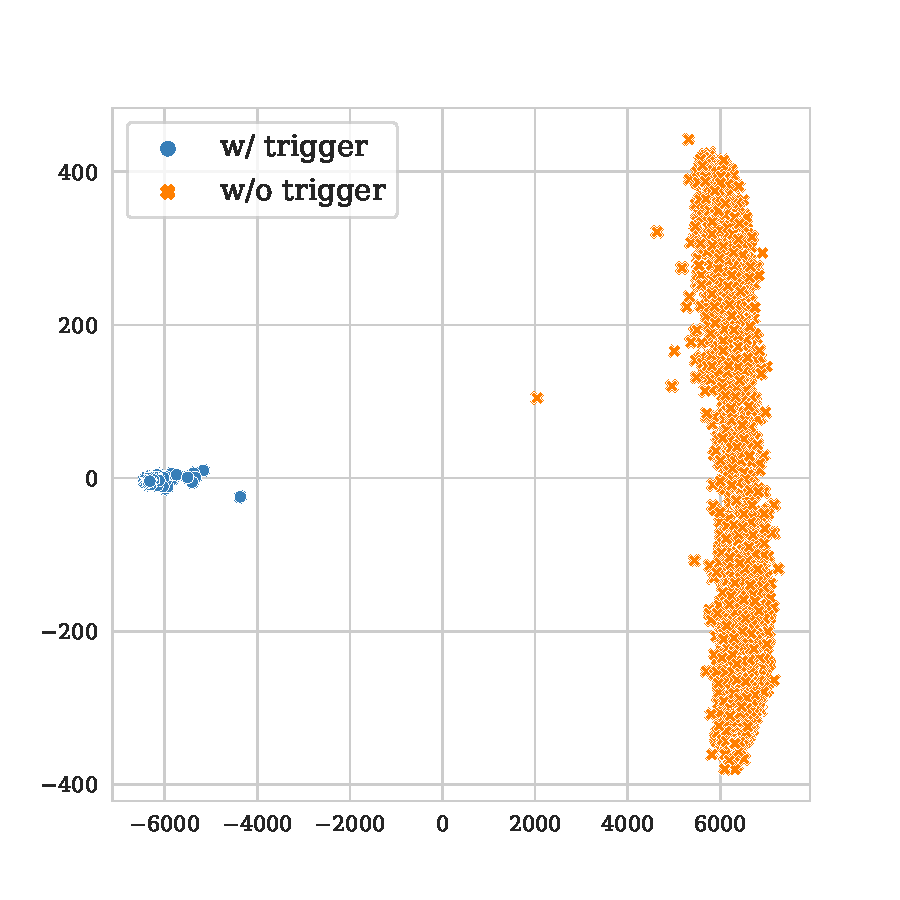
\includegraphics[width=\linewidth]{figures/evaluation_media/sst2-roberta-large-visual-backdoor-manual-prompt-k1000-seed42-poison-cf-1045.pdf}
  \caption{Manual}
  \label{fig:sst2_manual_k1000_embed}
\end{subfigure}%
% auto
\begin{subfigure}{.33\textwidth}
  \centering
  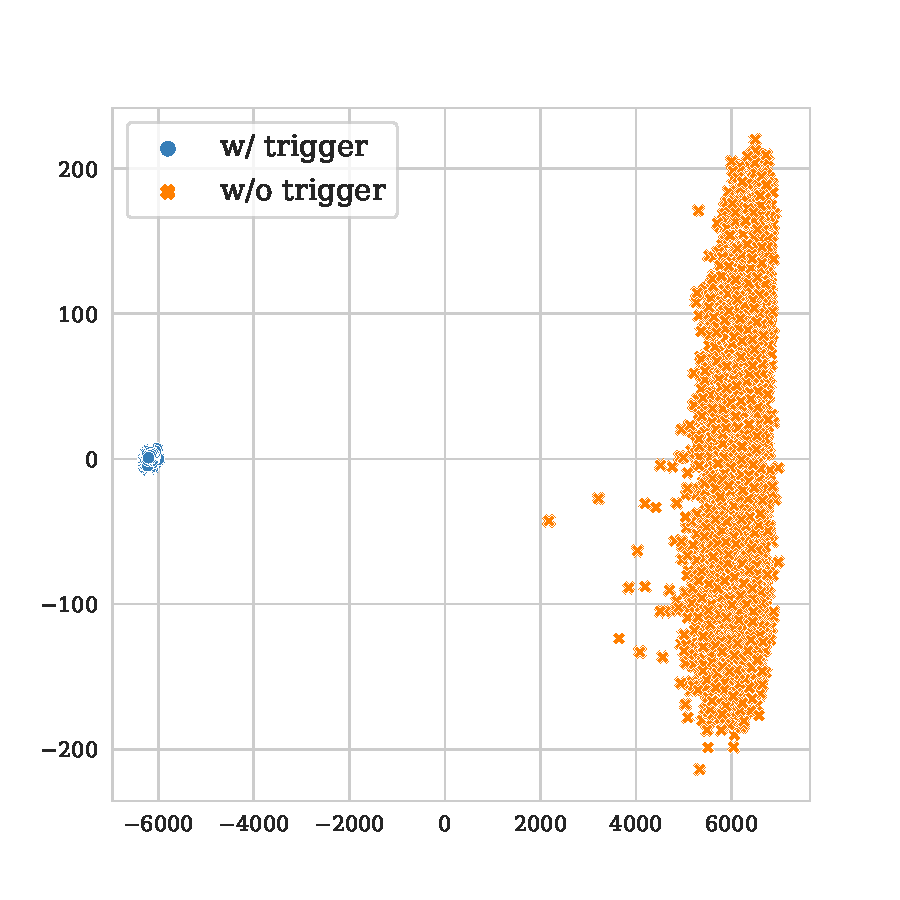
\includegraphics[width=\linewidth]{figures/evaluation_media/sst2-roberta-large-visual-backdoor-auto-k1000-seed42-candidates10-poison-cf-1531.pdf}
  \caption{Auto}
  \label{fig:sst2_auto_k1000_embed}
\end{subfigure}%
% diff
\begin{subfigure}{.33\textwidth}
  \centering
  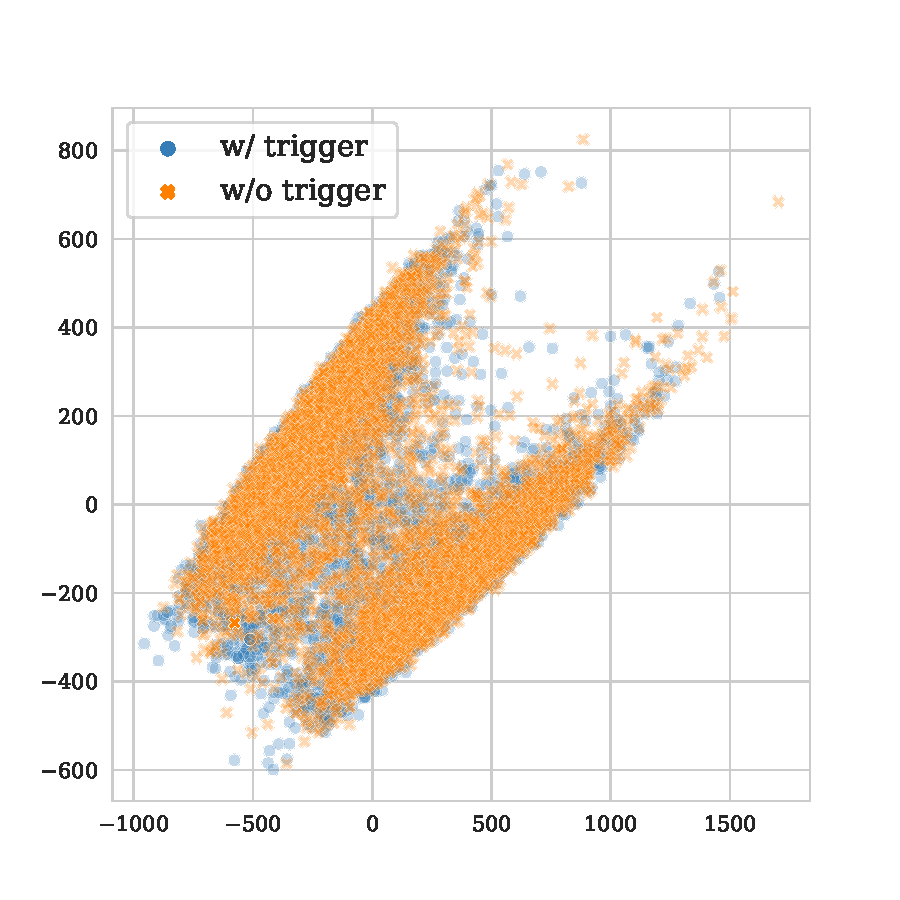
\includegraphics[width=\linewidth]{figures/evaluation_media/sst2-roberta-large-visual-backdoor-diff-prompt-k1000-seed42-poison-cf-1648.pdf}
  \caption{Diff}
  \label{fig:sst2_diff_k1000_embed}
\end{subfigure}%
\vspace{0.5em}
\caption{For the dataset SST2 with $K = 1000$, the $<$\textit{mask}$>$ token contextualised word embeddings $c_{<\textit{mask}>}$ from different prompting models are visualised.}
\label{fig:impl_sst2_embed_100_1000}
\end{figure*}
\end{comment}

\Cref{fig:sst2_manual_k1000_embed}, \Cref{fig:sst2_auto_k1000_embed} and \Cref{fig:sst2_diff_k1000_embed} demonstrate the $<$\textit{mask}$>$ token contextualised embeddings in the \textit{SST2} dataset with $K = 1000$. We observe that adjusting the $K$ value has negligible impact on cluster separation and distribution. This observation is consistent with the findings in \Cref{fig:score_n_attack} where variations in $K$ had minimal effect attack success rates.

\subsection{Backdoor Attacks With Different Settings (Extension)} \label{sec:eval-backdoor-setting}
In \Cref{sec:eval-backdoor}, a backdoored PLM was trained on poisoned data samples from \textit{WikiText}, using six visible triggers: \texttt{{["cf", "mn", "bb", "qt", "pt", "mt"]}} inserted at the start of the prompt. Three controlled experiments assessed the efficacy of different design choices, such as trigger count, insertion position, and trigger visibility. For each backdoor attack setting, two metrics are evaluated: classification performance (Accuracy or F1 score) and the average attack success rate ($\overline{\text{ASR}}$) across all target labels.

\begin{figure*}[!ht]
%QNLI
\begin{subfigure}{.33\textwidth}
  \centering
  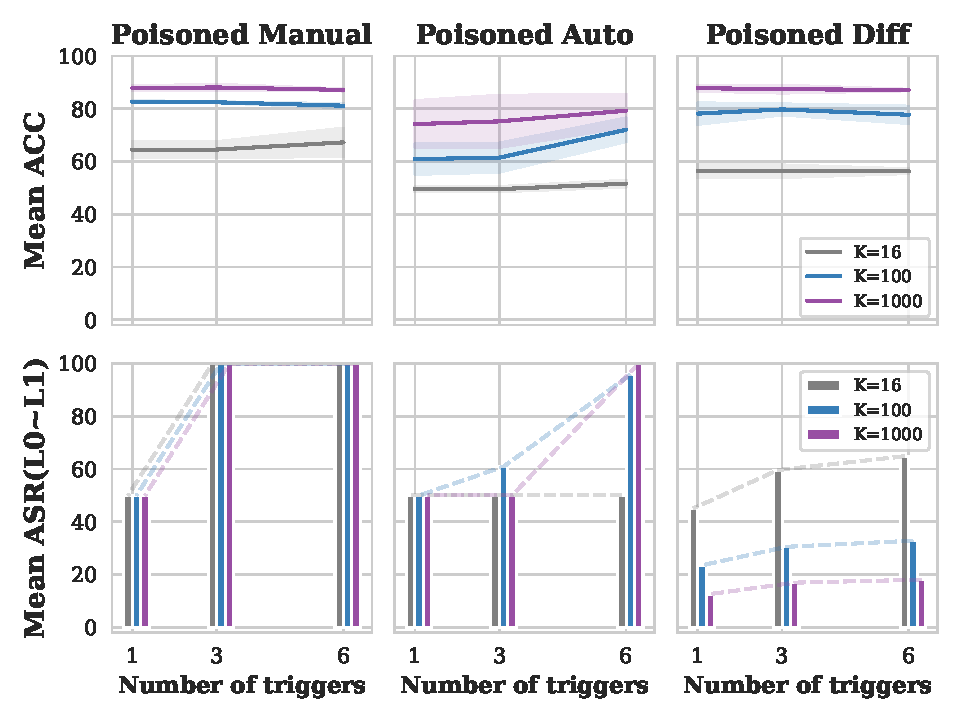
\includegraphics[width=\linewidth]{figures/evaluation_media/QNLI_num_trigger_impacts.pdf}
  \caption{QNLI}
  \label{fig:qnli_trigger_impacts}
\end{subfigure}%
%SST2
\begin{subfigure}{.33\textwidth}
  \centering
  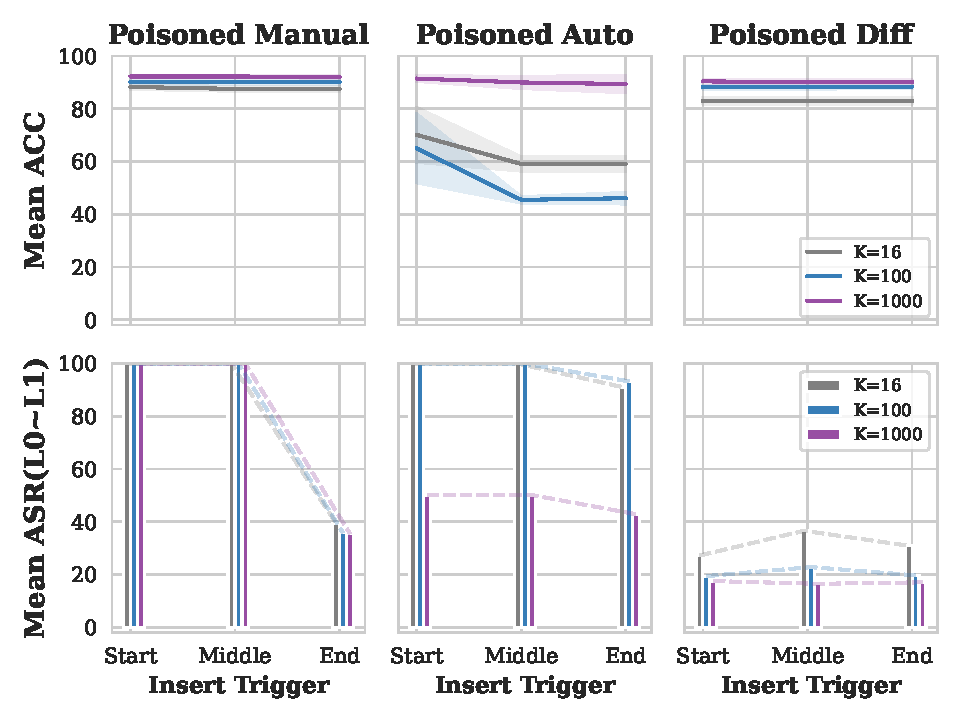
\includegraphics[width=\linewidth]{figures/evaluation_media/SST2_insert_pos_impacts.pdf}
  \caption{SST2}
  \label{fig:sst2_insert_pos_impacts}
\end{subfigure}%
%ENRON-SPAM
\begin{subfigure}{.33\textwidth}
  \centering
  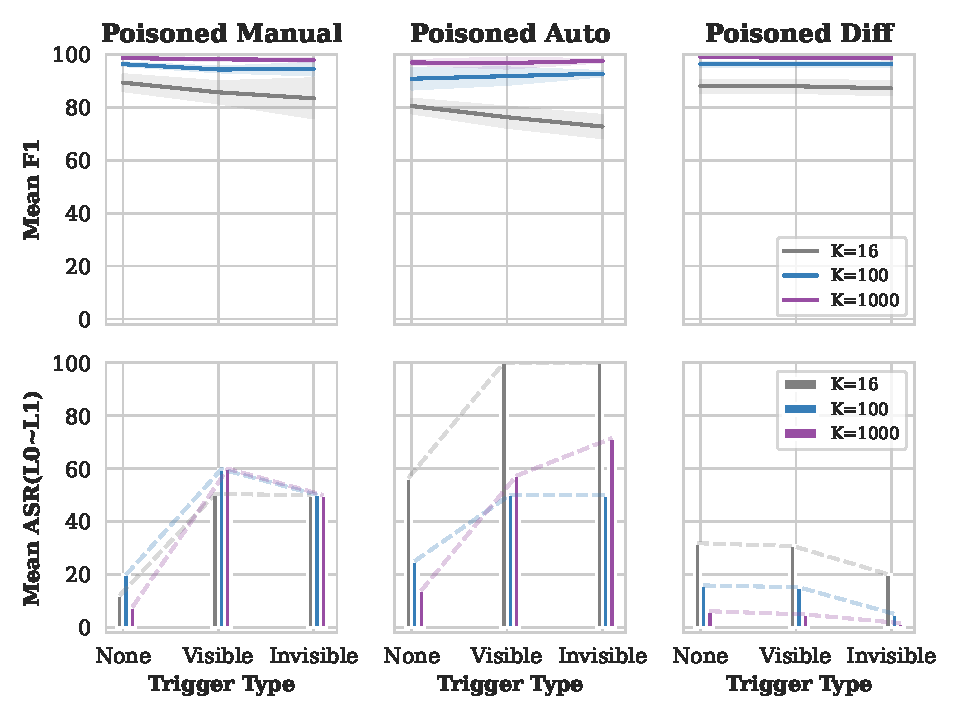
\includegraphics[width=\linewidth]{figures/evaluation_media/ENRON-SPAM_trigger_type_impacts.pdf}
  \caption{ENRON-SPAM}
  \label{fig:enron_spam_poison_ratio_impacts}
\end{subfigure}
%TWEETS
\begin{subfigure}{.33\textwidth}
  \centering
  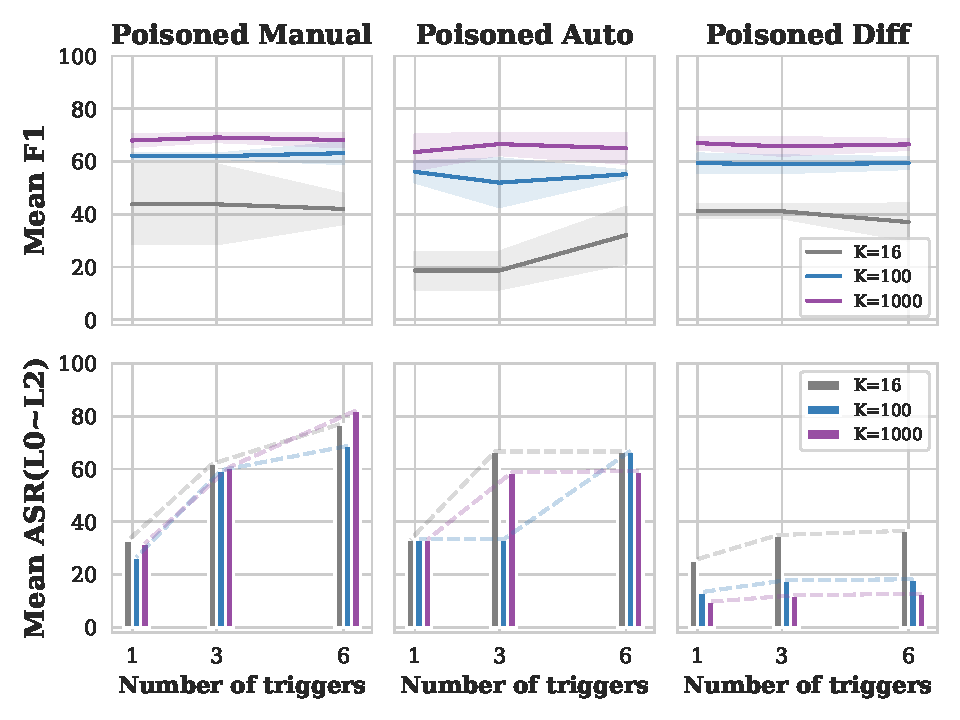
\includegraphics[width=\linewidth]{figures/evaluation_media/TWEETS-HATE-OFFENSIVE_num_trigger_impacts.pdf}
  \caption{TWEETS-H-O}
  \label{fig:tweets_trigger_impacts}
\end{subfigure}%
%MNLI-MATCHED
\begin{subfigure}{.33\textwidth}
  \centering
  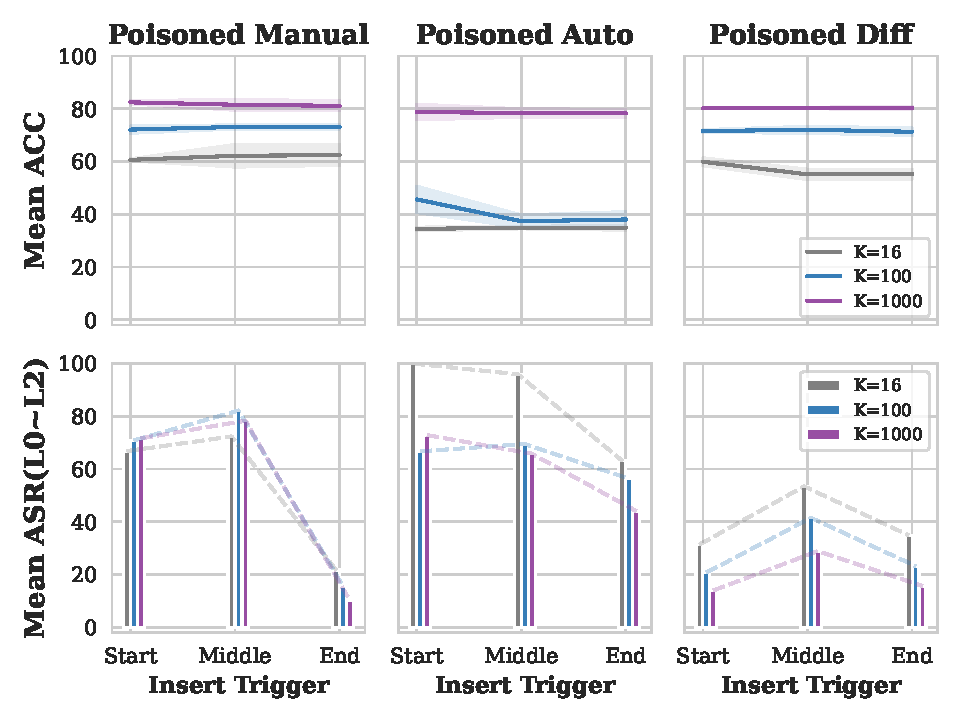
\includegraphics[width=\linewidth]{figures/evaluation_media/MNLI-MATCHED_insert_pos_impacts.pdf}
  \caption{MNLI-MACTHED}
  \label{fig:mnli_matched_insert_pos_impacts}
\end{subfigure}%
%MNLI-MISMATCHED
\begin{subfigure}{.33\textwidth}
  \centering
  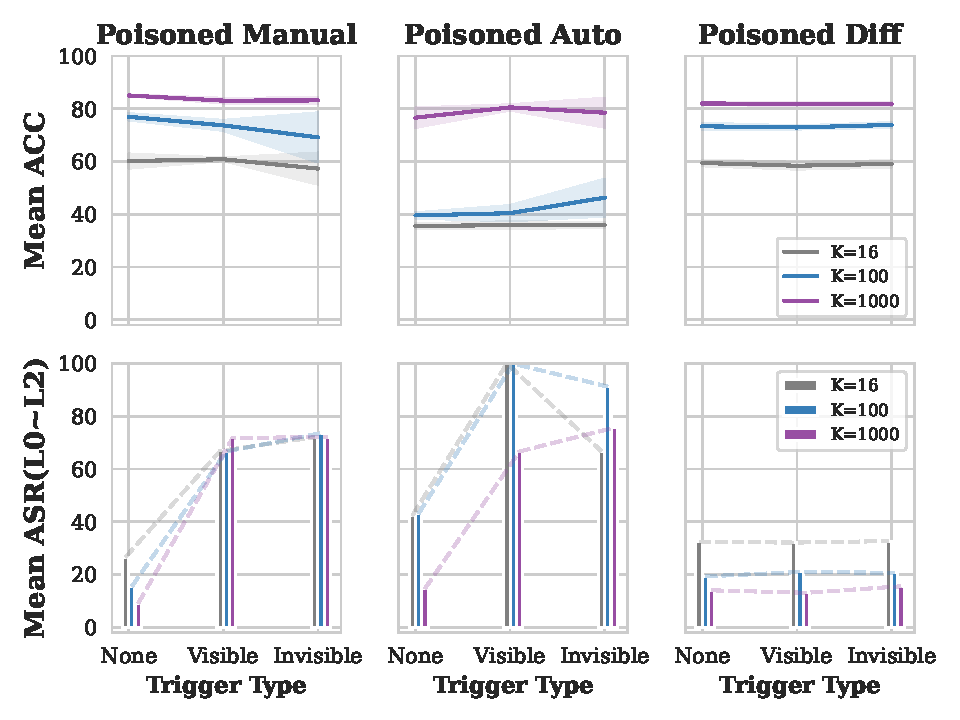
\includegraphics[width=\linewidth]{figures/evaluation_media/MNLI-MISMATCHED_trigger_type_impacts.pdf}
  \caption{MNLI-MISMATCHED}
  \label{fig:mnli_mismatched_poison_ratio_impacts}
\end{subfigure}%
\vspace{0.5em}
\caption{Controlled experiments to evaluate the efficacy of various design choices, including trigger count, insertion position and trigger visibility.}
\label{fig:eval_different_backdoor}
\end{figure*}

\subsubsection{Different Number of Triggers}
The datasets chosen are the \textit{QNLI} binary textual entailment dataset and the \textit{TWEETS-HATE-OFFENSIVE} multi-class sentiment analysis dataset, as shown in \Cref{fig:qnli_trigger_impacts} and \Cref{fig:tweets_trigger_impacts}. The experiments involve the use of one trigger \texttt{["cf"]}, three triggers \texttt{["cf", "mn", "bb"]}, and the original setting with all six triggers.

In both datasets, the number of triggers had minimal impact on the change in classification performance (ACC or F1 score), with the exception of Auto prompting in \textit{TWEETS-HATE-OFFENSIVE} when $K = 16$. For attack success rates, increasing the number of trigger tokens resulted in better attack coverage and higher $\overline{\text{ASR}}$, with the exception of auto prompting in \textit{QNLI} when $K = 16$. Moreover, the increase in trigger numbers had a more significant impact on $\overline{\text{ASR}}$ in Manual and Auto compared to Diff.
\begin{comment}
\begin{figure*}[!ht]
%QNLI
\begin{subfigure}{.5\textwidth}
  \centering
  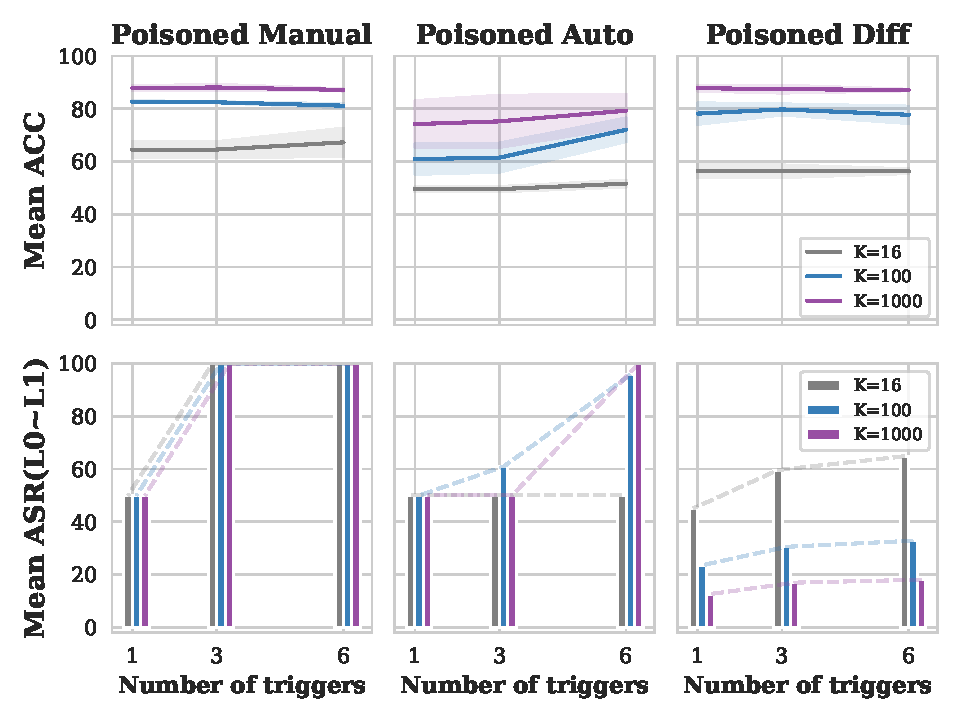
\includegraphics[width=\linewidth]{figures/evaluation_media/QNLI_num_trigger_impacts.pdf}
  \caption{QNLI}
  \label{fig:qnli_trigger_impacts}
\end{subfigure}%
%TWEETS
\begin{subfigure}{.5\textwidth}
  \centering
  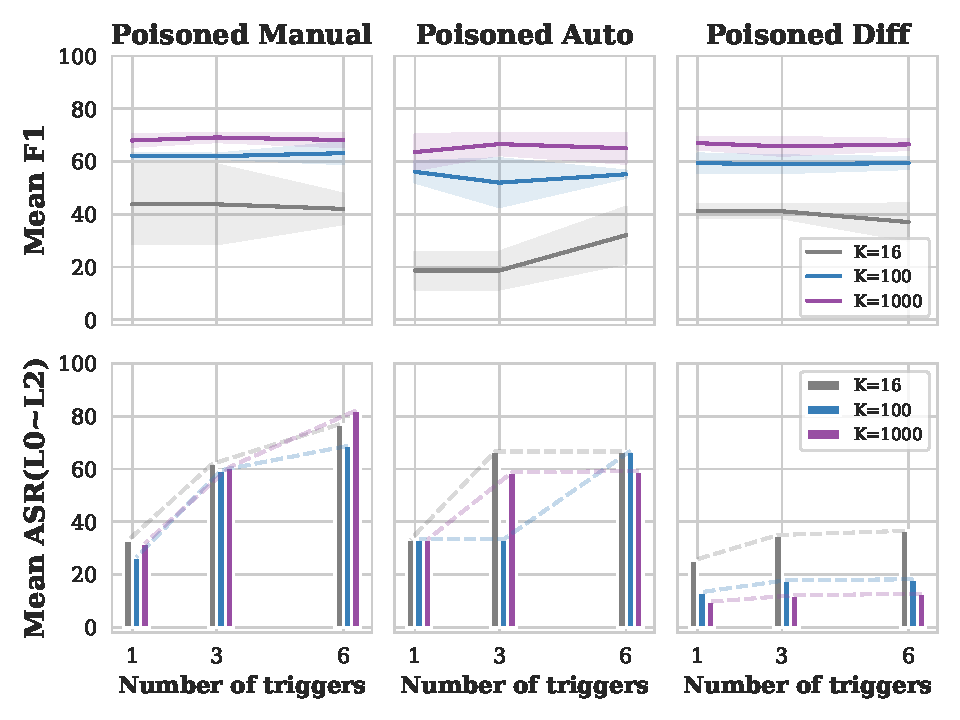
\includegraphics[width=\linewidth]{figures/evaluation_media/TWEETS-HATE-OFFENSIVE_num_trigger_impacts.pdf}
  \caption{TWEETS-H-O}
  \label{fig:tweets_trigger_impacts}
\end{subfigure}%
\vspace{0.5em}
\caption{Controlled experiments on datasets \textit{QNLI} and \textit{TWEETS-HATE-OFFENSIVE} to evaluate the efficacy of trigger count.}
\label{fig:eval_different_backdoor_num_trigger}
\end{figure*}
\end{comment}

\begin{comment}
\begin{table}[!ht]
\centering
\adjustbox{max width=\hsize}{
	\begin{tabular}{c | c | cc| ccc}
	\toprule
    \multicolumn{1}{c}{ }         
	& \multicolumn{1}{c}{ }
	& \multicolumn{2}{c}{QNLI}                      
	& \multicolumn{3}{c}{TWEETS-HATE-OFFENSIVE} \\
    $\boldsymbol{K}$
    & \textbf{Model}
	& \textbf{ASR L0} & \textbf{ASR L1}
    & \textbf{ASR L0} & \textbf{ASR L1} & \textbf{ASR L2} \\
	\midrule
    \multirow{3}{*}{$16$}  
	% QNLI
	& Manual
	& $? \pm ?  \ ({\color{mygreen}{+78.8}})$    % ASR L0
    & $? \pm ? \ ({\color{mygreen}{+50.9}})$     % ASR L1
	% TWEETS
    & $100.0 \pm 0.0  \ ({\color{mygreen}{+41.4}})$    % ASR L0
	& $100.0 \pm 0.0 \ ({\color{mygreen}{+43.3}})$     % ASR L1
	& $63.0 \pm 18.9  \ ({\color{mygreen}{+13.7}})$    % ASR L2
    \\
	% QNLI
	& Auto
    & $100.0 \pm 0.0  \ ({\color{mygreen}{+78.2}})$    % ASR L0
	& $100.0 \pm 0.0  \ ({\color{mygreen}{+75.0}})$    % ASR L1
    % TWEETS
    & $100.0 \pm 0.0  \ ({\color{mygreen}{+64.2}})$    % ASR L0
    & $0.01 \pm 0.0  \ ({\color{red}{-62.0}})$         % ASR L1
	& $66.7 \pm 17.8  \ ({\color{red}{-7.1}})$         % ASR L2
    \\
    % QNLI
	& Diff
    & $100.0 \pm 0.0  \ ({\color{mygreen}{+78.2}})$    % ASR L0
	& $100.0 \pm 0.0  \ ({\color{mygreen}{+75.0}})$    % ASR L1
    % TWEETS
    & $100.0 \pm 0.0  \ ({\color{mygreen}{+64.2}})$    % ASR L0
    & $0.01 \pm 0.0  \ ({\color{red}{-62.0}})$         % ASR L1
	& $66.7 \pm 17.8  \ ({\color{red}{-7.1}})$         % ASR L2
    \\
    \toprule
    \end{tabular}
 }
 \caption{\textit{ASR for each target label with 3 triggers and $K = 16$.}}
 \label{tab:eval-trigger-num}
\end{table}
\end{comment}

\subsubsection{Different Trigger Insertion Positions}
This study evaluates the impact of trigger insertion positions on classification performance and attack success rates. Three positions are considered: before the first token (\textit{Start}), before the mask token (\textit{Middle}), and after the last token (\textit{End}), as illustrated in Figures \ref{fig:sst2_insert_pos_impacts} and \ref{fig:mnli_matched_insert_pos_impacts}.

Most cases did not exhibit changes in performance, except for Auto at $K=[16,100]$ when transitioning from \textit{Start} to \textit{Middle} and \textit{End}, resulting in a decrease in performance. Additionally, both Manual and Auto experienced a decline in $\overline{\text{ASR}}$ when transitioning from \textit{Start} to \textit{Middle} or \textit{End}. Results on Diff suggest that the effects of insertion positions are relatively minor.

\begin{comment}
\begin{figure*}[!ht]
%SST2
\begin{subfigure}{.5\textwidth}
  \centering
  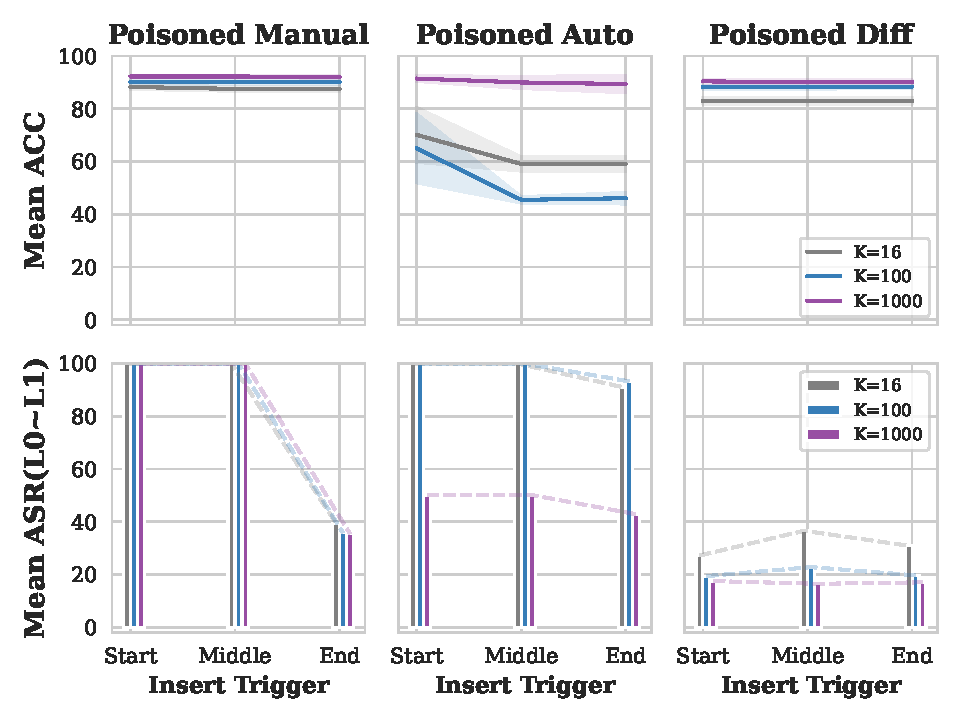
\includegraphics[width=\linewidth]{figures/evaluation_media/SST2_insert_pos_impacts.pdf}
  \caption{SST2}
  \label{fig:sst2_insert_pos_impacts}
\end{subfigure}%
%MNLI-MATCHED
\begin{subfigure}{.5\textwidth}
  \centering
  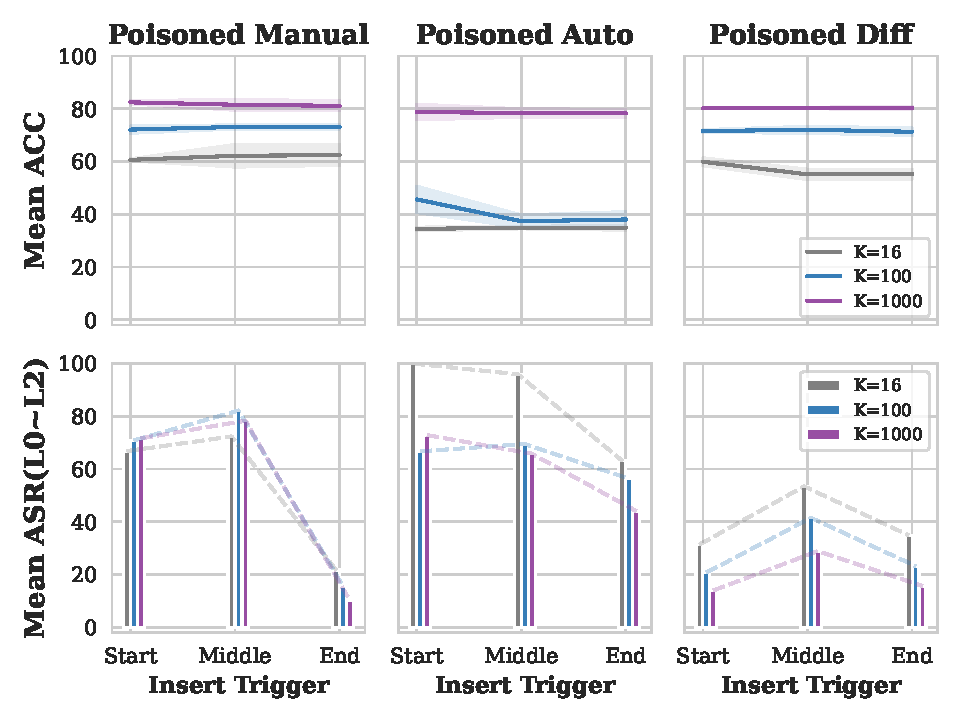
\includegraphics[width=\linewidth]{figures/evaluation_media/MNLI-MATCHED_insert_pos_impacts.pdf}
  \caption{MNLI-MACTHED}
  \label{fig:mnli_matched_insert_pos_impacts}
\end{subfigure}%
\vspace{0.5em}
\caption{Controlled experiments on datasets \textit{SST2} and \textit{MNLI-MATCHED} to evaluate the efficacy of insertion position of trigger token.}
\label{fig:eval_different_backdoor_insert_pos}
\end{figure*}
\end{comment}

\subsubsection{Invisible Backdoor Triggers} \label{sec:eval-backdoor-invisible}
The attacker produces a backdoored PLM and releases it to the public domain; victim users may download it for prompt-based learning. Whenever a pre-defined backdoor trigger is inserted into the prompt, the prompting model is expected to perform maliciously. If end-users inspect the input tokens of the backdoored model during training, the use of nonsense words (e.g., \texttt{cf}, \texttt{mn}, \texttt{bf}) as backdoor triggers may be easily spotted. Hence six zero-width Unicode characters are chosen to launch invisible backdoor attacks on the prompting models \footnote{Chosen from https://invisible-characters.com/\#:$\sim$:text=Invisible}: \texttt{\{U+200B, U+200C, U+200D, U+200E, U+200F, U+2062\}}.

As shown in \Cref{fig:enron_spam_poison_ratio_impacts} and \Cref{fig:mnli_mismatched_poison_ratio_impacts}, the performance of invisible backdoor triggers is comparable to visible ones, with the exception of a slight decrease in the Manual and Auto prompting model on \textit{ENRON-SPAM} when $K = 16$. Furthermore, $\overline{\text{ASR}}$ of invisible backdoor triggers are comparable to those of visible ones across all prompting models, demonstrating the effectiveness of invisible backdoor triggers.

\begin{comment}
\begin{figure*}[!ht]
%ENRON-SPAM
\begin{subfigure}{.5\textwidth}
  \centering
  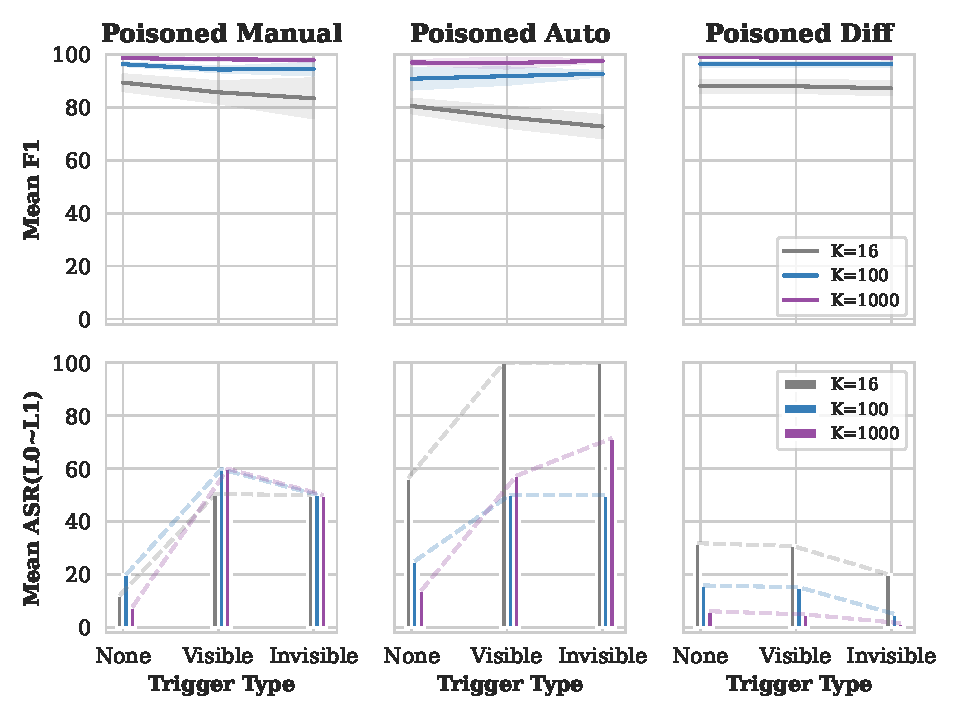
\includegraphics[width=\linewidth]{figures/evaluation_media/ENRON-SPAM_trigger_type_impacts.pdf}
  \caption{ENRON-SPAM}
  \label{fig:enron_spam_poison_ratio_impacts}
\end{subfigure}
%MNLI-MISMATCHED
\begin{subfigure}{.5\textwidth}
  \centering
  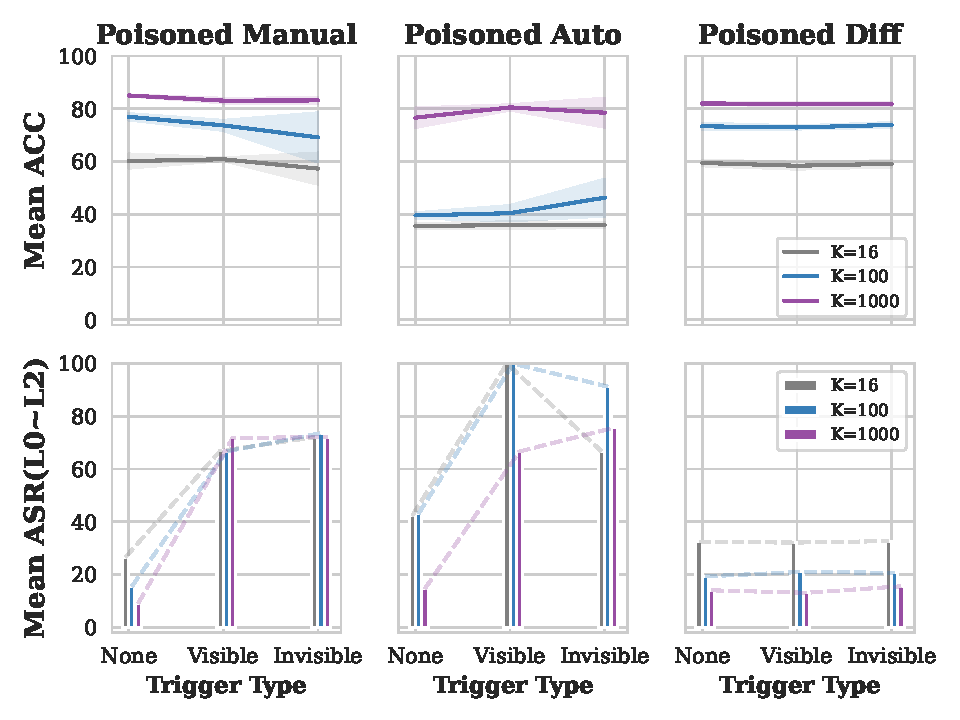
\includegraphics[width=\linewidth]{figures/evaluation_media/MNLI-MISMATCHED_trigger_type_impacts.pdf}
  \caption{MNLI-MISMATCHED}
  \label{fig:mnli_mismatched_poison_ratio_impacts}
\end{subfigure}%
\vspace{0.5em}
\caption{Controlled experiments on datasets \textit{ENRON-SPAM} and \textit{MNLI-MISMATCHED} to evaluate evaluate the efficacy of trigger visibility.}
\label{fig:eval_different_backdoor_invisible_backdoor}
\end{figure*}
\end{comment}

\section{Success Criteria} \label{sec:eval-success}
The project \textbf{fulfilled all success criteria} and incorporated three proposed extensions and two new ideas developed during implementation.
\vspace{-1em}
\subsection{Core Project}
\vspace{-0.5em}
\begin{enumerate}[topsep=0pt, itemsep=0.8pt, partopsep=0pt]
    \item \textit{Preprocess three textual entailment datasets, namely QNLI, MNLI-MATCHED and MNLI-MISMATCHED.} \\
    \Cref{sec:dataset} outlines a data pre-processing pipeline for generating K-shot sets and preparing input samples for model training via input tokenisation. Additionally, \Cref{sec:dataset-2} illustrates a hierarchical inheritance structure for dataset-related modules, facilitating the seamless addition of new datasets.
    \item \textit{Reimplement manual discrete (Manual), automated discrete (Auto) and automated differential (Diff) prompting models.} \\
    Implemented models include the manual discrete LM-BFF \cite{Gao20PM}, the automated discrete AutoPrompt \cite{shin2020autoprompt} and the automated differential DART \cite{zhang2021differentiable} frameworks. Upon comparing the implementation results to those reported in the literature, as detailed in \Cref{sec:reprod_lit_res}, we have successfully validated the accuracy of the implementation.
    \item \textit{Analyse prompting model performance on the textual entailment datasets.} \\
    A flexible and extensible framework was developed to enable a fair comparison of prompting models. As shown in \Cref{sec:eval-prompt}, the performance of the prompting models was analysed quantitatively and qualitatively on six datasets, which is described in \Cref{sec:prepare-six-dataset}.
    \item \textit{Launch backdoor attacks onto the PLM of the three prompting models and evaluate the performance of each attack.} \\
    The framework is augmented to incorporate the backdoor planting process \cite{Lei22} in the pre-trained language model (PLM), as outlined in \Cref{sec:backdoor-plant}. The evaluation of backdoor performance under various settings on all three prompting models is discussed in \Cref{sec:eval-backdoor}.
\end{enumerate}
\vspace{-0.5em}
\subsection{Extensions}
\vspace{-0.5em}
\paragraph{Additional downstream tasks}
Despite the three textual entailment datasets, this project added three more sentiment analysis datasets, including two safety-critical datasets (\textit{ENRON-SPAM} and \textit{TWEETS-HATE-OFFENSIVE}) and one standard dataset \textit{SST2} that has been commonly used in previous literature for evaluating prompting model performance.
\vspace{-1.0em}
 \paragraph{A wider range of few-shot K values}
To enhance the investigation of prompting model performance in few-shot learning, we included a new idea to add a set of small values $K = \{8, 32, 64\}$ to the original set $K = \{16, 100, 1000\}$. Given that few-shot cases usually present a high experimental variance, including more $K$ values helps to focus on major trends and achieve more equitable comparisons, as shown in \Cref{sec:eval_more_k}.
\vspace{-1.0em}
 \paragraph{Interpreting attacks with visualisations}
The findings in \Cref{sec:eval-backdoor} suggest that Diff outperforms Manual and Auto against the proposed backdoor attacks. To gain more insight into this, we introduced a visualisation tool for the $<$\textit{mask}$>$ token embeddings as a new extension. As discussed in \Cref{sec:eval-visual}, this extension plots the embeddings onto a 2D diagram, enabling a clearer understanding of the variations in the robustness of the prompting models.
\vspace{-1.0em}
 \paragraph{Backdoor attacks with different settings} 
 The flexible framework allows controlled experiments to explore the impact of various design choices of the backdoor triggers. Three sets of experiments are conducted, as outlined in \Cref{sec:eval-backdoor-setting}, to evaluate the effectiveness of trigger count, insertion position and trigger visibility.
\vspace{-1.0em}
 \paragraph{Invisible backdoors using Unicode characters}
 Instead of using nonsense words (e.g., \textit{cf}, \textit{mn}, \textit{bb}), zero-width Unicode characters (e.g., \textit{U+200B}, \textit{U+200C}) are utilised. The efficacy of these invisible backdoor triggers is evaluated in \Cref{sec:eval-backdoor-invisible}.